\chapter{Recursive Datatype Definitions: The Domain Package}
\label{ch:domain}

\section{Introduction}

Datatype definitions are a standard feature of many functional programming languages. A datatype definition is a way for a user to specify a new type, by explicitly enumerating all the ways that values of that type may be constructed. A datatype definition, then, consists of a list of \emph{constructors}, each of which may take zero or more arguments of specified types.

For example, in Haskell we might define a datatype \hs{OptInts}, consisting of optional pairs of integers; values of type \hs{OptInts} include \hs{None}, as well as pairs like \hs{Pair 3 5}. (And because we can write non-terminating expressions in Haskell, type \hs{OptInts} actually includes the special value $\bot$ as well.)
%
\begin{hscode}
data OptInts = None | Pair Int Int
\end{hscode}
%
Datatypes may also be \emph{recursive}, where the type being defined appears on the right-hand side of the definition. Below is an example of a binary tree datatype, where the \hs{Branch} constructor takes two other subtrees as arguments. Values of type \hs{BinTree} include \hs{Tip}, \hs{Branch Tip Tip}, and \hs{Branch Tip (Branch Tip Tip)}; \hs{Branch} constructors may be nested to any depth.
%
\begin{hscode}
data BinTree = Tip | Branch BinTree BinTree
\end{hscode}
%
Datatypes can also have \emph{type parameters}, such as this type of lists where the element type is specified by the parameter \hs{a}. Values include \hs{Cons 3 (Cons 5 Nil)}, which has type \hs{List Int}.
%
\begin{hscode}
data List a = Nil | Cons a (List a)
\end{hscode}

\paragraph{Isabelle/HOL Datatype package.}

The \textsc{Datatype} package implements these kinds of recursive datatype definitions for Isabelle/HOL. It provides an input syntax that looks very much like the Haskell definitions.
%
\begin{isacode}
datatype opt_ints = None | Pair "int" "int"
\end{isacode}
\unmedskip
\begin{isacode}
datatype bintree = Tip | Branch "bintree" "bintree"
\end{isacode}
\unmedskip
\begin{isacode}
datatype 'a list = Nil | Cons "'a" "'a list"
\end{isacode}
%
However, unlike Haskell, the \textsc{Datatype} package lives and works in a world of inductive data and total functions. Types defined by the \textsc{Datatype} package include precisely those values that can be built up using finite combinations of constructor functions; nothing more, nothing less. In particular, they do not include \isa{\<bottom>}, or any infinite values.

\paragraph{Isabelle/HOLCF Domain package.}

The \textsc{Domain} package provides a similar datatype facility for HOLCF, in a world of cpos, bottoms, infinite values, and continuous functions. Like the \textsc{Datatype} package, it also supports a syntax that looks very much like Haskell:
%
\begin{isacode}
domain opt_ints = None | Pair "int lift" "int lift"
\end{isacode}
\unmedskip
\begin{isacode}
domain bintree = Tip | Branch "bintree" "bintree"
\end{isacode}
\unmedskip
\begin{isacode}
domain 'a list = Nil | Cons "'a" "'a list"
\end{isacode}
%
But unlike the \textsc{Datatype} package, the \textsc{Domain} package produces types that are pointed cpos: The constructors are continuous functions, and \isa{\<bottom>} is an element of every datatype. Types defined by the \textsc{Domain} package may or may not include partial and infinite values, depending on whether the user decides to make the datatype lazy. (Laziness is the default for datatypes in Haskell, but not for strict functional languages like ML.) For example, the lazy version of \isa{bintree} shown below includes both finite and infinite values, including an infinite value consisting of nothing but \isa{Branch} constructors all the way down.

\begin{isacode}
domain bintree = Tip | Branch (lazy "bintree") (lazy "bintree")
\end{isacode}

The HOLCF \textsc{Domain} package was originally created by David von Oheimb in 1997 \cite{Oheimb97}, after which it became an integral part of \HOLCF{99} \cite{hol+lcf}. Since the initial version, the code has undergone a fairly significant amount of modification and improvement by the present author. The main purpose of this chapter is to document the current state of the implementation, and explain the ideas behind all the new code that was not present in the original.

The original \textsc{Domain} package relied on a rather dubious implementation technique: Instead of following the definitional approach, and actually constructing recursive datatypes, it relied on axioms to help define new datatypes. Specifically, each new datatype required three new axioms to be declared; further definitions and proofs were then based on these. In all the years since \HOLCF{99}, the \textsc{Domain} package has continued to use axioms to support its definitions, although many of the intervening changes to the code have been motivated by the goal of eliminating the reliance on axioms.

At last, in \HOLCF{11} the \textsc{Domain} package now has two instantiations---an axiomatic mode (kept for backward compatibility) and a new definitional mode. This chapter describes the operation of the axiomatic version. However, only a small fraction of the code is specific to the axiomatic mode, so most of this chapter is equally applicable to both versions. Relative to the axiomatic mode, the definitional mode requires a significant amount of extra theoretical machinery to implement, which will be built up in the course of Chapters \ref{ch:powerdomain} and \ref{ch:universal}.

\paragraph{Contributions.}

Much of the material presented in this chapter is just a reworking of von Oheimb's original \textsc{Domain} package implementation \cite{Oheimb97}. Since the \HOLCF{99} version, many of the present author's improvements to the package have been incremental. However there are a few new features that stand out:

\begin{itemize*}
\item New modular code organization, to isolate the axiom-generating components
\item Efficient method for proving exhaustiveness of constructors, using rewriting
\item Notion of \emph{decisive} take functions for recognizing finite-valued domains
\item Support for indirect-recursive domain definitions
\item Integration with the \textsc{Fixrec} package
\item Numerous speed-ups, making large datatype definitions feasible
\end{itemize*}

\paragraph{Overview.}

The remainder of this chapter consists of two main parts. First, we describe the \textsc{Domain} package from a user's point of view, explaining the various kinds of domain specifications it is possible to write, and the relevant constants and theorems the package generates (\S\ref{sec:domain-features}). Next we cover the implementation of the \textsc{Domain} package, showing how it is organized into modules, and how each module works (\S\ref{sec:domain-implementation}). The chapter concludes with a short summary and discussion of the problems caused by axioms, and previews the eventual solution to these problems (\S\ref{sec:domain-discussion}).

\section{Domain package features}
\label{sec:domain-features}

\subsection{Strict and lazy constructors}

The \textsc{Domain} package has an input syntax similar to the Isabelle/HOL \textsc{Datatype} package \cite{isabelle-tutorial}. The right-hand side of a domain definition consists of one or more constructors, each with zero or more argument types.

\begin{isacode}
domain 'a strictlist = nil | cons "'a" "'a strictlist"
\end{isacode}

Each domain definition produces constructors with continuous function types. For example, defining \isa{'a strictlist} as shown yields the function \isa{cons} with type \isa{'a \<rightarrow> 'a strictlist \<rightarrow> 'a strictlist}. Constructor functions are strict by default, so \isa{cons\<cdot>\<bottom>\<cdot>s = \<bottom>} and \isa{cons\<cdot>a\<cdot>\<bottom> = \<bottom>}. Constructors can be made non-strict in specified arguments using the \isa{lazy} keyword.
%
\indexdefx{domain 'a stream}
\begin{isacode}
domain 'a stream = SNil | SCons "'a" (lazy "'a stream")
\end{isacode}
%
Note that making the recursive argument lazy causes type \isa{'a stream} to include infinite values, in constrast with \isa{'a strictlist}, whose values are all finite.

The \textsc{Domain} package also generates a collection of rewrite rules about the constructors, which are added to the simplifier.
%
\begin{isacode}
"SCons\<cdot>\<bottom>\<cdot>s = \<bottom>"
"SNil \<noteq> \<bottom>"
"SCons\<cdot>a\<cdot>s = \<bottom> \<longleftrightarrow> a = \<bottom>"
"a \<noteq> \<bottom> \<Longrightarrow> SCons\<cdot>a\<cdot>s \<sqsubseteq> SCons\<cdot>a'\<cdot>s' \<longleftrightarrow> a \<sqsubseteq> a' \<and> s \<sqsubseteq> s'"
"a \<noteq> \<bottom> \<Longrightarrow> SCons\<cdot>a\<cdot>s = SCons\<cdot>a'\<cdot>s' \<longleftrightarrow> a = a' \<and> s = s'"
"SNil \<notsqsubseteq> SCons\<cdot>a'\<cdot>s'"
"SCons\<cdot>a\<cdot>s \<sqsubseteq> SNil \<longleftrightarrow> a = \<bottom>"
"SNil \<noteq> SCons\<cdot>a'\<cdot>s'"
"SCons\<cdot>a\<cdot>s \<noteq> SNil"
"compact SNil"
"\<lbrakk>compact a; compact s\<rbrakk> \<Longrightarrow> compact (SCons\<cdot>a\<cdot>s)"
\end{isacode}

In addition to the simplification rules, the \textsc{Domain} package also generates theorems asserting that the constructors are exhaustive. The generated theorems follow a naming scheme similar to the Isabelle/HOL \textsc{Datatype} package, where each theorem is qualified by the name of the relevant type. The two logically equivalent theorems below follow the same pattern as the similarly-named theorems generated by \textsc{Datatype}, except that they also include cases for \isa{\<bottom>} and strict constructor functions.
%
\indexthmx{stream.nchotomy}
\begin{isacode}
theorem stream.nchotomy:
  "y = \<bottom> \<or> y = SNil \<or> (\<exists>a s. y = SCons\<cdot>a\<cdot>s \<and> a \<noteq> \<bottom>)"
\end{isacode}
\unmedskip
\indexthmx{stream.exhaust}
\begin{isacode}
theorem stream.exhaust:
  "\<lbrakk>y = \<bottom> \<Longrightarrow> P; y = SNil \<Longrightarrow> P; \<And>a s. \<lbrakk>y = SCons\<cdot>a\<cdot>s; a \<noteq> \<bottom>\<rbrakk> \<Longrightarrow> P\<rbrakk> \<Longrightarrow> P"
\end{isacode}

The \textsc{Domain} package registers \isa{stream.exhaust} as the default case analysis rule for type \isa{'a stream}. This means proof methods like \isa{apply (cases y)} can be used on a stream variable \isa{y}, without having to explicitly name rule \isa{stream.exhaust}.

\subsection{Case expressions}

The \textsc{Domain} package configures Isabelle's parser to allow case expressions on each new datatype. This case syntax is supported by \emph{case combinators}. For example, with the \isa{'a stream} domain, the case expression \isa{\<case> x of SNil \<Rightarrow> y | SCons\<cdot>a\<cdot>s \<Rightarrow> z} translates to \isa{stream_case\<cdot>y\<cdot>(\<Lambda> a s. z)\<cdot>x}. The case combinator \isa{stream_case}, which has type \isa{'b \<rightarrow> ('a \<rightarrow> 'a stream \<rightarrow> 'b) \<rightarrow> 'a stream \<rightarrow> 'b}, satisfies the following simplification rules:

\begin{isacode}
theorem stream.case_rews [simp]:
  "stream_case\<cdot>f1\<cdot>f2\<cdot>\<bottom> = \<bottom>"
  "stream_case\<cdot>f1\<cdot>f2\<cdot>SNil = f1"
  "a \<noteq> \<bottom> \<Longrightarrow> stream_case\<cdot>f1\<cdot>f2\<cdot>(SCons\<cdot>a\<cdot>s) = f2\<cdot>a\<cdot>s"
\end{isacode}

\subsection{Mixfix syntax}

In Isabelle, a \emph{mixfix} declaration specifies custom syntax for parsing and pretty printing; infix syntax is a special case for functions of two arguments. The \textsc{Domain} package supports mixfix declarations for data constructors. For example, we can specify syntax for \isa{SNil} and an infix operator for the \isa{SCons} constructor, like this:
%
\begin{isacode}
domain 'a stream =
  SNil ("<>") | SCons "'a" (lazy "'a stream") (infixr "##" 60)
\end{isacode}
%
Now \isa{<>} is defined as alternative syntax for \isa{SNil}, and \isa{a ## s} abbreviates \isa{SCons\<cdot>a\<cdot>s}.

Mixfix declarations can also be given for the type constructors themselves. For example:
%
\begin{isacode}
domain ('a, 'b) either (infixl ":+:" 20) = Left (lazy "'a") | Right (lazy "'b")
\end{isacode}
%
This introduces the type notation \isa{'a :+: 'b} as an abbreviation for \isa{('a, 'b) either}.

\subsection{Selector functions}

Each constructor argument in a domain declaration may be given an optional selector name. For example, for our \isa{'a stream} datatype we can label the arguments of \isa{SCons} as \isa{head} and \isa{tail}:

\begin{isacode}
domain 'a stream = SNil | SCons (head :: "'a") (lazy tail :: "'a stream")
\end{isacode}
%
The \textsc{Domain} package then defines two selector functions: \isa{head :: 'a stream \<rightarrow> 'a} and \isa{tail :: 'a stream \<rightarrow> 'a stream}. When applied to the correct constructor, each selector function projects out the desired argument; applied to any other constructor, the selector returns \isa{\<bottom>}. Accordingly, the package derives the following rewrite rules, which are added to the simplifier.

\begin{isacode}
theorem stream.sel_rews [simp]:
  "head\<cdot>\<bottom> = \<bottom>"
  "tail\<cdot>\<bottom> = \<bottom>"
  "head\<cdot>SNil = \<bottom>"
  "tail\<cdot>SNil = \<bottom>"
  "head\<cdot>(SCons\<cdot>a\<cdot>s) = a"
  "a \<noteq> \<bottom> \<Longrightarrow> tail\<cdot>(SCons\<cdot>a\<cdot>s) = s"
\end{isacode}

\subsection{Discriminator functions}

The \textsc{Domain} package automatically defines a discriminator function for each data constructor. Each discriminator function returns a lifted boolean, depending on its argument: \isa{TT} if its argument is the correct constructor, \isa{FF} for a different constructor, and \isa{\<bottom>} if its argument is \isa{\<bottom>}. For example, when defining type \isa{'a stream}, the package generates \isa{is_SNil :: 'a stream \<rightarrow> tr} and \isa{is_SCons :: 'a stream \<rightarrow> tr}. These functions satisfy the following rules, which are declared to the simplifier.

\begin{isacode}
theorem stream.dis_rews [simp]:
  "is_SNil\<cdot>\<bottom> = \<bottom>"
  "is_SCons\<cdot>\<bottom> = \<bottom>"
  "is_SNil\<cdot>x = \<bottom> \<longleftrightarrow> x = \<bottom>"
  "is_SCons\<cdot>x = \<bottom> \<longleftrightarrow> x = \<bottom>"
  "is_SNil\<cdot>SNil = TT"
  "a \<noteq> \<bottom> \<Longrightarrow> is_SNil\<cdot>(SCons\<cdot>a\<cdot>s) = FF"
  "is_SCons\<cdot>SNil = FF"
  "a \<noteq> \<bottom> \<Longrightarrow> is_SCons\<cdot>(SCons\<cdot>a\<cdot>s) = TT"
\end{isacode}

\subsection{Fixrec package support}

The \textsc{Domain} package generates a match combinator for each data constructor, and registers them for use with the \textsc{Fixrec} package. Most of the details are irrelevant as far as users are concerned; the important thing is that after defining a datatype with the \textsc{Domain} package, users can write function definitions over that datatype using \textsc{Fixrec}.

\subsection{Take functions}

Each datatype defined by the \textsc{Domain} package gets its own \emph{take function}, which is actually a chain of functions that return finite approximations of their input values. These take functions are a bit like the Haskell function \hs{take} for lists, in that \isa{take (Suc n)} applied to a constructor maps \isa{take n} over that constructor's recursive arguments. However, unlike the Haskell \hs{take} function, \isa{take 0} is undefined (i.e., \isa{\<bottom>}). In this way, the HOLCF take functions are exactly like the generic \emph{approx} functions discussed by Hutton and Gibbons \cite{Hutton01}.

For the \isa{'a stream} datatype, the \textsc{Domain} package defines a function \isa{stream_take} whose type is \isa{nat \<Rightarrow> 'a stream \<rightarrow> 'a stream}. The defining equations below are added as default simplification rules.
%
\begin{isacode}
  "stream_take 0 = \<bottom>"
  "stream_take n\<cdot>\<bottom> = \<bottom>"
  "stream_take (Suc n)\<cdot>SNil = SNil"
  "stream_take (Suc n)\<cdot>(SCons\<cdot>a\<cdot>s) = SCons\<cdot>a\<cdot>(stream_take n\<cdot>s)"
\end{isacode}
%\begin{isacode}
%theorem stream.take_0 [simp]: "stream_take 0 = \<bottom>"
%\end{isacode}
%\unmedskip
%\begin{isacode}
%theorem stream.take_strict [simp]: "stream_take n\<cdot>\<bottom> = \<bottom>"
%\end{isacode}
%\unmedskip
%\begin{isacode}
%theorem stream.take_rews [simp]:
%  "stream_take (Suc n)\<cdot>SNil = SNil"
%  "stream_take (Suc n)\<cdot>(SCons\<cdot>a\<cdot>s) = SCons\<cdot>a\<cdot>(stream_take n\<cdot>s)"
%\end{isacode}
%
The package also derives a few more theorems from the definition of \isa{stream_take}, which can also be useful for simplification:
%
\indexthmx{stream.chain_take}
\begin{isacode}
theorem stream.chain_take [simp]: "chain (\<lambda>n. stream_take n)"
\end{isacode}
\unmedskip
\indexthmx{stream.take_below}
\begin{isacode}
theorem stream.take_below: "stream_take n\<cdot>x \<sqsubseteq> x"
\end{isacode}
\unmedskip
\indexthmx{stream.take_take}
\begin{isacode}
theorem stream.take_take:
  "stream_take m\<cdot>(stream_take n\<cdot>x) = stream_take (min m n)\<cdot>x"
\end{isacode}

In practice, take functions are usually used for low-level induction proofs. The \textsc{Domain} package generates a \emph{reach axiom} (in two equivalent forms) stating that the least upper bound of the chain of take functions is the identity. The principle of \emph{take induction} (rule \isa{stream.take_induct}) is a direct corollary of the reach axiom.

\indexthmx{stream.lub_take}
\begin{isacode}
theorem stream.lub_take: "(\<Squnion>n. stream_take n) = ID"
\end{isacode}
\unmedskip
\indexthmx{stream.reach}
\begin{isacode}
theorem stream.reach: "(\<Squnion>n. stream_take n\<cdot>x) = x"
\end{isacode}
\unmedskip
\indexthmx{stream.take_induct}
\begin{isacode}
theorem stream.take_induct: "\<lbrakk>adm P; \<And>n. P (stream_take n\<cdot>x)\<rbrakk> \<Longrightarrow> P x"
\end{isacode}

The \emph{take lemma} is another reasoning principle derived from the reach axiom. This lets users show that two (possibly infinite) values are equal, by showing that the finite values returned by the take functions are equal.
%
\indexthmx{stream.take_lemma}
\begin{isacode}
theorem stream.take_lemma:
  "(\<And>n. stream_take n\<cdot>x = stream_take n\<cdot>y) \<Longrightarrow> x = y"
\end{isacode}
%
A variation of the take lemma, specific to lazy lists, was originally popularized by Bird and Wadler \cite{BirdWadler1988}. The take lemma generated by the \textsc{Domain} package is actually identical to the generic ``approximation lemma'' described by Hutton and Gibbons \cite{Hutton01}. An example of a proof using the take lemma can be found in the case study in Chapter~\ref{ch:case-domain}.

\subsection{Induction rules}

In addition to the low-level take induction rules, the \textsc{Domain} package also generates some high-level induction principles in terms of the constructor functions.

\begin{isacode}
theorem stream.finite_induct:
  "\<lbrakk>P \<bottom>; P SNil; \<And>a s. \<lbrakk>a \<noteq> \<bottom>; P s\<rbrakk> \<Longrightarrow> P (SCons\<cdot>a\<cdot>s)\<rbrakk>
    \<Longrightarrow> P (stream_take n\<cdot>x)"
\end{isacode}
%
To be able to conclude that a property holds for \emph{all} streams, including infinite ones, the full induction rule adds an admissibility requirement.
%
\begin{isacode}
theorem stream.induct:
  "\<lbrakk>adm P; P \<bottom>; P SNil; \<And>a s. \<lbrakk>a \<noteq> \<bottom>; P s\<rbrakk> \<Longrightarrow> P (SCons\<cdot>a\<cdot>s)\<rbrakk> \<Longrightarrow> P x"
\end{isacode}
%
For mutually recursive domain definitions, the \textsc{Domain} package generates a mutual induction rule for proving properties of both types simultaneously.
%
\indexdefx{domain 'a list1}
\indexdefx{domain 'a list2}
\begin{isacode}
domain 'a list1 = Nil1 | List2 (lazy "'a list2")
  and 'a list2 = Cons2 (lazy "'a") (lazy "'a list1")
\end{isacode}
\unmedskip
\indexthmx{list1_list2.induct}
\begin{isacode}
theorem list1_list2.induct:
  "\<lbrakk>adm P1; adm P2; P1 \<bottom>; P1 Nil1; \<And>list2. P2 list2 \<Longrightarrow> P1 (List2\<cdot>list2);
    P2 \<bottom>; \<And>a list1. P1 list1 \<Longrightarrow> P2 (Cons2\<cdot>a\<cdot>list1)\<rbrakk> \<Longrightarrow> P1 x1 \<and> P2 x2"
\end{isacode}

The \textsc{Domain} package declares the high-level induction rules as the default induction rules for their types. This means that, for example, the proof method \isa{apply (induct s)} will use rule \isa{stream.induct} if \isa{s} is a variable of type \isa{'a stream}. Likewise, the simultaneous induction method \isa{apply (induct x and y)} will automatically use rule \isa{list1_list2.induct} if \isa{x} and \isa{y} have the appropriate types.

\subsection{Finite-valued domains}

Some datatypes, like \isa{'a strictlist} below, contain only finite values because recursion only occurs via strict constructor arguments. For such datatypes, the \textsc{Domain} package can generate induction rules without an admissibility condition. This includes both the low-level take induction principle, and the ordinary high-level induction rule.
%
\indexdefx{domain 'a strictlist}
\begin{isacode}
domain 'a strictlist = nil | cons "'a" "'a strictlist"
\end{isacode}
\unmedskip
\indexthmx{strictlist.take_induct}
\begin{isacode}
theorem strictlist.take_induct: "(\<And>n. P (strictlist_take n\<cdot>x)) \<Longrightarrow> P x"
\end{isacode}
\unmedskip
\indexthmx{strictlist.induct}
\begin{isacode}
theorem strictlist.induct:
  "\<lbrakk>P \<bottom>; P nil; \<And>a s. \<lbrakk>a \<noteq> \<bottom>; s \<noteq> \<bottom>; P s\<rbrakk> \<Longrightarrow> P (cons\<cdot>a\<cdot>s)\<rbrakk> \<Longrightarrow> P x"
\end{isacode}
%
The \textsc{Domain} package can also recognize finite-valued domains in mutually recursive definitions.

\subsection{Coinduction}

The \textsc{Domain} package implements the principle of \emph{coinduction} for recursive domains, following the design described by Pitts~\cite{Pitts1994}. The main concept underlying coinduction is the \emph{bisimulation} relation: A binary relation \isa{R} is a bisimulation if any two values related by \isa{R} are either both \isa{\<bottom>}, or else they are the same constructor, with their arguments again related by \isa{R}.
%
\begin{isacode}
definition stream_bisim :: "('a stream \<Rightarrow> 'a stream \<Rightarrow> bool) \<Rightarrow> bool"
  where "stream_bisim R \<equiv> (\<forall>x y. R x y \<longrightarrow>
    (x = \<bottom> \<and> y = \<bottom>) \<or>
    (x = SNil \<and> y = SNil) \<or>
    (\<exists>a s a' s'. a = a' \<and> R s s' \<and> x = SCons\<cdot>a\<cdot>s \<and> y = SCons\<cdot>a'\<cdot>s'))"
\end{isacode}
%
The principle of coinduction states that any two values related by any bisimulation relation must be equal.
%
\begin{isacode}
theorem stream.coinduct: "\<lbrakk>stream_bisim R; R x y\<rbrakk> \<Longrightarrow> x = y"
\end{isacode}
%
A good exposition of the proof technique of coinduction, as used for lazy lists, can be found in Gibbons and Hutton \cite{Gibbons2005}. The implementation of coinduction for recursive domains has changed little since the \HOLCF{99} \textsc{Domain} package, and we will not be using coinduction further in this dissertation.

\subsection{Indirect recursion}

In all the recursive domain definitions shown so far, occurrences of recursive types have only appeared directly as constructor arguments. But it is also possible for a recursive type to occur \emph{indirectly}, under one or more other type constructors. For example, in the following definition of \isa{bintree}, the argument type of the \isa{Branch} constructor contains recursive occurrences of \isa{bintree} within a strict product.
%
\begin{isacode}
domain bintree = Tip | Branch "bintree \<otimes> bintree"
\end{isacode}
%
Unlike the \HOLCF{99} \textsc{Domain} package, the \HOLCF{11} version now supports such indirect-recursive domain definitions. One user-visible consequence of indirect recursion is that the rewrite rules for take functions mention \emph{map combinators}:
%
\begin{isacode}
"bintree_take (Suc n)\<cdot>(Branch\<cdot>x) =
  Branch\<cdot>(sprod_map\<cdot>(bintree_take n)\<cdot>(bintree_take n)\<cdot>x)"
\end{isacode}
%
Here \isa{sprod_map} is a combinator that maps each of two functions over the respective elements of a strict pair. There are similar map combinators for a few other type constructors that the \textsc{Domain} package also knows about; these are shown in Fig.~\ref{fig:domain-map-combinators}. In Chapter~\ref{ch:universal} when we talk about the definitional \textsc{Domain} package, we will see how to make this list extensible, in a sound way.

\begin{figure}
\indexdef{prod_map}
\begin{isacode}
definition prod_map :: "('a \<rightarrow> 'b) \<rightarrow> ('c \<rightarrow> 'd) \<rightarrow> 'a \<times> 'c \<rightarrow> 'b \<times> 'd"
  where "prod_map = (\<Lambda> f g (x, y). (f\<cdot>x, g\<cdot>y))"
\end{isacode}
\unmedskip
\indexdef{sprod_map}
\begin{isacode}
definition sprod_map :: "('a \<rightarrow> 'b) \<rightarrow> ('c \<rightarrow> 'd) \<rightarrow> 'a \<otimes> 'c \<rightarrow> 'b \<otimes> 'd"
  where "sprod_map = (\<Lambda> f g. (:x y:). (:f\<cdot>x, g\<cdot>y:)))"
\end{isacode}
\unmedskip
\indexdef{ssum_map}
\begin{isacode}
definition ssum_map :: "('a \<rightarrow> 'b) \<rightarrow> ('c \<rightarrow> 'd) \<rightarrow> 'a \<oplus> 'c \<rightarrow> 'b \<oplus> 'd"
  where "ssum_map = (\<Lambda> f g. sscase\<cdot>(sinl oo f)\<cdot>(sinr oo g))"
\end{isacode}
\unmedskip
\indexdef{u_map}
\begin{isacode}
definition u_map :: "('a \<rightarrow> 'b) \<rightarrow> 'a u \<rightarrow> 'b u"
  where "u_map = (\<Lambda> f. fup\<cdot>(up oo f))"
\end{isacode}
\unmedskip
\indexdef{cfun_map}
\begin{isacode}
definition cfun_map :: "('b \<rightarrow> 'a) \<rightarrow> ('c \<rightarrow> 'd) \<rightarrow> ('a \<rightarrow> 'c) \<rightarrow> ('b \<rightarrow> 'd)"
  where "cfun_map = (\<Lambda> a b f x. b\<cdot>(f\<cdot>(a\<cdot>x)))"
\end{isacode}
\caption{Map combinators for various HOLCF types}
\label{fig:domain-map-combinators}
\end{figure}

For indirect-recursive domains, the \textsc{Domain} package still generates take induction rules, just as it does for any other domain definition. However, currently it does not produce high-level induction or coinduction rules. Formulating high-level induction rules for arbitrary indirect-recursive domains is still an experimental topic; we will have more to say about this in the case study in Chapter~\ref{ch:case-domain}.

%%%%%%%%%%%%%%%%%%%%%%%%%%%%%%%%%%%%%%%%%%%%%%%%%%

\section{Implementation}
\label{sec:domain-implementation}

The entire implementation of the \textsc{Domain} package is based on pairs of functions that form \emph{domain isomorphisms}. Each isomorphism relates the new ``abstract'' type, such as \isa{'a stream}, to a ``representation'' type built from strict sums and products, plus lifting to model laziness. For example, consider our lazy stream type:
%
\begin{isacode}
domain 'a stream = SNil | SCons (head :: "'a") (lazy tail :: "'a stream")
\end{isacode}
%
Here \isa{'a stream} is the abstract type and \isa{one \<oplus> ('a \<otimes> 'a stream\<^sub>\<bottom>)} is the representation type. The \textsc{Domain} package produces continuous \isa{abs} and \isa{rep} functions between these two types, which are analogous to the \isa{Abs} and \isa{Rep} functions produced by the \textsc{Typedef} package described in Chapter~\ref{ch:holcf}.
%
\begin{isacodes}
stream_abs :: "one \<oplus> ('a \<otimes> 'a stream\<^sub>\<bottom>) \<rightarrow> 'a stream"
stream_rep :: "'a stream \<rightarrow> one \<oplus> ('a \<otimes> 'a stream\<^sub>\<bottom>)"
\end{isacodes}
%
Together with standard operations on the strict sum, strict product, and lifting types, the \isa{abs} and \isa{rep} functions can be used to define all the necessary operations on new domain types---such as constructors, case combinators, and take functions. Most of the properties of these operations are derived from the \emph{isomorphism axioms}, which assert that the \isa{abs} and \isa{rep} functions are each other's inverses.

Since \HOLCF{99}, the \textsc{Domain} package has undergone a significant reorganization to make the code more modular. The diagram in Fig.~\ref{fig:domain-implementation} shows the main components, and how information is passed between them. The new organization offers multiple benefits. For example, all code dealing with constructor functions is now isolated in components in the bottom half of the diagram. The other modules, located in the top half, only need to know about domain isomorphisms, and never see any information about constructor functions. These modules can then have simpler interfaces, and also fewer dependencies on the other components, making maintenance easier.

\begin{figure}
\begin{center}
\begin{singlespace}
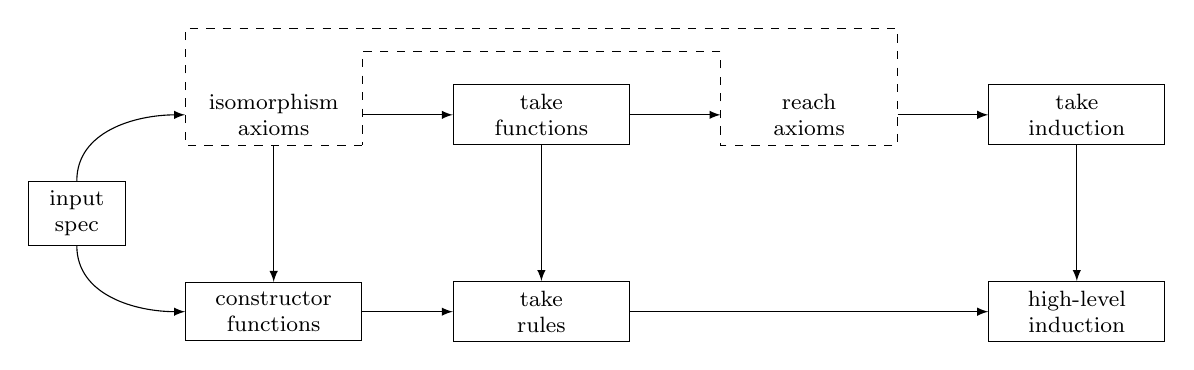
\begin{tikzpicture}
  [ axiom/.style={rectangle, text width=2cm, text centered, font=\footnotesize}
  , proof/.style={rectangle, text width=2cm, text centered, font=\footnotesize, draw}
  , >=latex]
  \node (0) at (-2.5, 1.25) [rectangle, text width=1cm, text centered, font=\footnotesize, draw] {input\\spec};
  \node (1) at (0.0, 2.5) [axiom] {isomorphism\\axioms};
  \node (2) at (3.4, 2.5) [proof] {take\\functions};
  \node (3) at (6.8, 2.5) [axiom] {reach\\axioms};
  \node (4) at (10.2, 2.5) [proof] {take\\induction};
  \node (5) at (0.0, 0.0) [proof] {constructor\\functions};
  \node (6) at (3.4, 0.0) [proof] {take\\rules};
  \node (7) at (10.2, 0.0) [proof] {high-level\\induction};
  \draw [->] (0.north) to [out=90, in=180] (1.west);
  \draw [->] (1) -- (2);
  \draw [->] (2) -- (3);
  \draw [->] (3) -- (4);
  \draw [->] (0.south) to [out=270, in=180] (5.west);
  \draw [->] (1) -- (5);
  \draw [->] (5) -- (6);
  \draw [->] (2) -- (6);
  \draw [->] (6) -- (7);
  \draw [->] (4) -- (7);
  \draw [dashed]
    (1.south east) -- (1.south west) -- (1.north west) --
    (1.west |- 0,3.6) -- (3.east |- 0,3.6) -- (3.south east) -- (3.south west) --
    (3.west |- 0,3.3) -- (1.east |- 0,3.3) -- (1.south east) -- cycle;
%    (1.west |- 0,3.6) -- (4.east |- 0,3.6) -- (4.east |- 0,3.3) --
%    (3.east |- 0,3.3) -- (3.south east) -- (3.south west) --
%    (3.west |- 0,3.3) -- (1.east |- 0,3.3) -- (1.south east) -- cycle;
\end{tikzpicture}
\end{singlespace}
\end{center}
\caption{Domain package implementation schematic}
\label{fig:domain-implementation}
\end{figure}

Another benefit of the new modularization is the ability to swap out individual components. In particular, note that all code involved with generating axioms is contained within the pair of modules inside the dashed lines in Fig.~\ref{fig:domain-implementation}. With clear interfaces between these axiomatic modules and the rest of the \textsc{Domain} package, it will be possible to replace them with definitional versions at a later time, with minimal modifications to the rest of the system. We will come back to the definitional version of the \textsc{Domain} package in Chapter~\ref{ch:universal}.

Each module in Fig.~\ref{fig:domain-implementation} will be explained in more detail in one of the following sections. For each module, we will describe the definitions and proofs that are generated, as well as the ML record types that make up the interfaces.

\subsection{Input specification module}

%%%%%%%%%%%%%%%%%%%%%%%%%%%%%%%%%%%%%%%%%%%%%%%%%%

\begin{figure}
\begin{center}
\begin{minipage}{0.725\linewidth}

\emph{definition}:

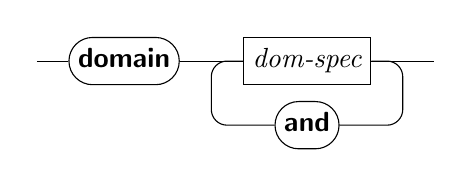
\begin{tikzpicture}
[ thin, draw, text height=1.5ex, text depth=0.4ex
, point/.style={coordinate}
, keyword/.style={rectangle, minimum size=6mm, rounded corners=3mm, draw, font=\bfseries\sffamily}
, terminal/.style={rectangle, minimum size=6mm, rounded corners=3mm, draw, font=\sffamily}
, nonterminal/.style={rectangle, minimum size=6mm, draw, font=\itshape}
, curve/.style={rounded corners=2mm}
]
\matrix[row sep=2mm, column sep=4mm] {
% First row:
\node (p0) [point] {}; &
\node (domain) [keyword] {domain}; &
\node (p3) [point] {}; &
\node (domspec) [nonterminal] {dom-spec}; &
\node (p4) [point] {}; &
\node (p5) [point] {}; \\
% Second row:
& & &
\node (and) [keyword] {and}; \\
};
\draw [curve] (p0) -- (domain) -- (domspec) -- (p5);
\draw [curve] (domspec) -- (p4) |- (and) -| (p3) -- (domspec);
\end{tikzpicture}

%%%%%%%%%%%%%%%%%%%%%%%%%%%%%%%%%%%%%%%%%%%%%%%%%%

\emph{dom-spec}:

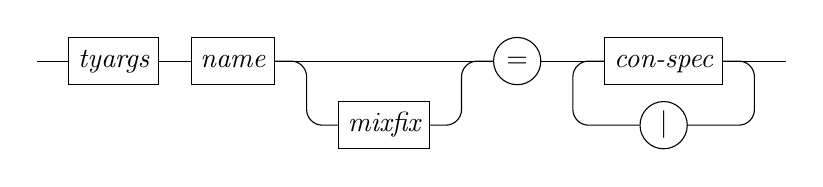
\begin{tikzpicture}
[ thin, draw, text height=1.5ex, text depth=0.4ex
, point/.style={coordinate}
, keyword/.style={rectangle, minimum size=6mm, rounded corners=3mm, draw, font=\bfseries\sffamily}
, terminal/.style={rectangle, minimum size=6mm, rounded corners=3mm, draw, font=\sffamily}
, nonterminal/.style={rectangle, minimum size=6mm, draw, font=\itshape}
, curve/.style={rounded corners=2mm}
]
\matrix[row sep=2mm, column sep=4mm] { 
% First row:
\node (p0) [point] {}; &
\node (tyargs) [nonterminal] {tyargs}; &
\node (name) [nonterminal] {name}; & 
\node (p3) [point] {}; & &
\node (p4) [point] {}; &
\node (equal) [terminal] {=}; &
\node (p5) [point] {}; &
\node (conspec) [nonterminal] {con-spec}; &
\node (p6) [point] {}; &
\node (p7) [point] {}; \\
% Second row:
& & & &
\node (mixfix) [nonterminal] {mixfix}; & & & &
\node (bar) [terminal] {\textbar}; \\
};
\draw [curve] (p0) -- (tyargs) -- (name) -- (equal) -- (conspec) -- (p7);
\draw [curve] (name) -- (p3) |- (mixfix) -| (p4) -- (equal);
\draw [curve] (conspec) -- (p6) |- (bar) -| (p5) -- (conspec);
\end{tikzpicture}

%%%%%%%%%%%%%%%%%%%%%%%%%%%%%%%%%%%%%%%%%%%%%%%%%%

\emph{tyargs}:

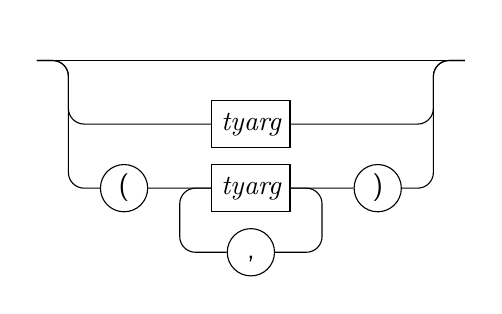
\begin{tikzpicture}
[ thin, draw, text height=1.5ex, text depth=0.4ex
, point/.style={coordinate}
, keyword/.style={rectangle, minimum size=6mm, rounded corners=3mm, draw, font=\bfseries\sffamily}
, terminal/.style={rectangle, minimum size=6mm, rounded corners=3mm, draw, font=\sffamily}
, nonterminal/.style={rectangle, minimum size=6mm, draw, font=\itshape}
, curve/.style={rounded corners=2mm}
]
\matrix[row sep=2mm, column sep=4mm] { 
% First row:
\node (p0) [point] {}; &
\node (p1) [point] {}; & & &
\useasboundingbox circle (3mm); & & &
\node (p2) [point] {}; &
\node (p3) [point] {}; \\
% Second row:
& & & &
\node (tyarg1) [nonterminal] {tyarg}; \\
% Third row:
& &
\node (lparen) [terminal] {(}; &
\node (p8) [point] {}; &
\node (tyarg2) [nonterminal] {tyarg}; &
\node (p9) [point] {}; &
\node (rparen) [terminal] {)}; \\
% Fourth row:
& & & &
\node (comma) [terminal] {,}; \\
};
\draw [curve] (p0) -- (p3);
\draw [curve] (p0) -- (p1) |- (tyarg1) -| (p2) -- (p3);
\draw [curve] (p0) -- (p1) |- (lparen) -- (tyarg2) -- (rparen) -| (p2) -- (p3);
\draw [curve] (tyarg2) -- (p9) |- (comma) -| (p8) -- (tyarg2);
\end{tikzpicture}

%%%%%%%%%%%%%%%%%%%%%%%%%%%%%%%%%%%%%%%%%%%%%%%%%%

\emph{tyarg}:

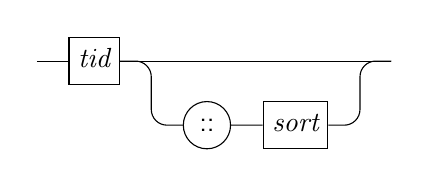
\begin{tikzpicture}
[ thin, draw, text height=1.5ex, text depth=0.4ex
, point/.style={coordinate}
, keyword/.style={rectangle, minimum size=6mm, rounded corners=3mm, draw, font=\bfseries\sffamily}
, terminal/.style={rectangle, minimum size=6mm, rounded corners=3mm, draw, font=\sffamily}
, nonterminal/.style={rectangle, minimum size=6mm, draw, font=\itshape}
, curve/.style={rounded corners=2mm}
]
\matrix[row sep=2mm, column sep=4mm] { 
% First row:
\node (p0) [point] {}; &
\node (tid) [nonterminal] {tid}; &
\node (p1) [point] {}; & & &
\node (p2) [point] {}; &
\node (p3) [point] {}; \\
% Second row:
& & &
\node (colon) [terminal] {::}; &
\node (sort) [nonterminal] {sort}; \\
};
\draw [curve] (p0) -- (tid) -- (p3);
\draw [curve] (tid) -- (p1) |- (colon) -- (sort) -| (p2) -- (p3);
\end{tikzpicture}

%%%%%%%%%%%%%%%%%%%%%%%%%%%%%%%%%%%%%%%%%%%%%%%%%%

\emph{con-spec}:

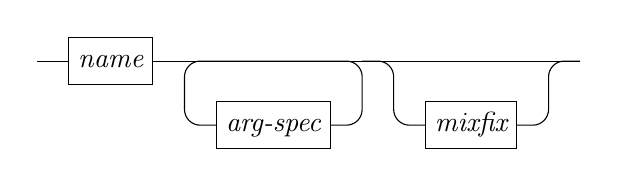
\begin{tikzpicture}
[ thin, draw, text height=1.5ex, text depth=0.4ex
, point/.style={coordinate}
, keyword/.style={rectangle, minimum size=6mm, rounded corners=3mm, draw, font=\bfseries\sffamily}
, terminal/.style={rectangle, minimum size=6mm, rounded corners=3mm, draw, font=\sffamily}
, nonterminal/.style={rectangle, minimum size=6mm, draw, font=\itshape}
, curve/.style={rounded corners=2mm}
]
\matrix[row sep=2mm, column sep=4mm] { 
% First row:
\node (p0) [point] {}; &
\node (name) [nonterminal] {name}; &
\node (p1) [point] {}; & &
\node (p2) [point] {}; &
\node (p3) [point] {}; & &
\node (p4) [point] {}; &
\node (p5) [point] {}; \\
% Second row:
& & &
\node (argspec) [nonterminal] {arg-spec}; & & &
\node (mixfix) [nonterminal] {mixfix}; \\
};
\draw [curve] (p0) -- (name) -- (p5);
\draw [curve] (argspec) -| (p2) -- (p1) |- (argspec);
\draw [curve] (p2) -- (p3) |- (mixfix) -| (p4) -- (p5);
\end{tikzpicture}

%%%%%%%%%%%%%%%%%%%%%%%%%%%%%%%%%%%%%%%%%%%%%%%%%%

\emph{arg-spec}:

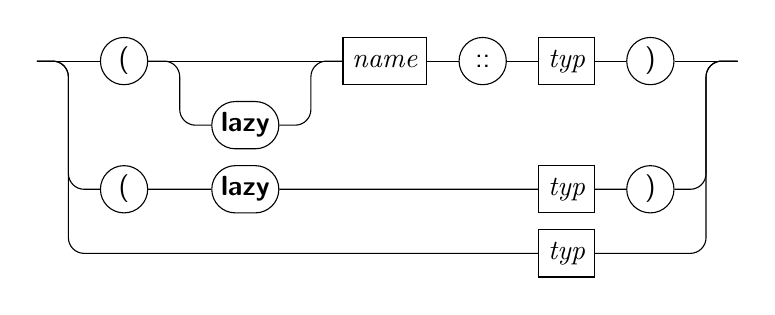
\begin{tikzpicture}
[ thin, draw, text height=1.5ex, text depth=0.4ex
, point/.style={coordinate}
, keyword/.style={rectangle, minimum size=6mm, rounded corners=3mm, draw, font=\bfseries\sffamily}
, terminal/.style={rectangle, minimum size=6mm, rounded corners=3mm, draw, font=\sffamily}
, nonterminal/.style={rectangle, minimum size=6mm, draw, font=\itshape}
, curve/.style={rounded corners=2mm}
]
\matrix[row sep=2mm, column sep=4mm] { 
% First row:
\node (p0) [point] {}; &
\node (p1) [point] {}; &
\node (lparen1) [terminal] {(}; &
\node (p2) [point] {}; & &
\node (p3) [point] {}; &
\node (name) [nonterminal] {name}; &
\node (colon) [terminal] {::}; &
\node (typ1) [nonterminal] {typ}; &
\node (rparen1) [terminal] {)}; &
\node (p4) [point] {}; &
\node (p5) [point] {}; \\
% Second row:
& & & &
\node (lazy1) [keyword] {lazy}; \\
% Third row:
& &
\node (lparen2) [terminal] {(}; & &
\node (lazy2) [keyword] {lazy}; & & & &
\node (typ2) [nonterminal] {typ}; &
\node (rparen2) [terminal] {)}; \\
% Fourth row:
& & & & & & & &
\node (typ3) [nonterminal] {typ}; \\
};
\draw [curve] (p0) -- (lparen1) -- (name) -- (colon) -- (typ1) -- (rparen1) -- (p5);
\draw [curve] (lparen1) -- (p2) |- (lazy1) -| (p3) -- (name);
\draw [curve] (p0) -- (p1) |- (lparen2) -- (lazy2) -- (typ2) -- (rparen2) -| (p4) -- (p5);
\draw [curve] (p0) -- (p1) |- (typ3) -| (p4) -- (p5);
\end{tikzpicture}

\end{minipage}
\end{center}

\caption{Input syntax for {\domain} package}
\label{fig:domain-input-syntax}
\end{figure}

%%%%%%%%%%%%%%%%%%%%%%%%%%%%%%%%%%%%%%%%%%%%%%%%%%

The input-specification module of the \textsc{Domain} package starts by parsing its input according to the grammar shown in Fig.~\ref{fig:domain-input-syntax}. The input consists of one or more domain specifications, each of which has a type on the left-hand side, and a list of constructor specifications on the right. Each constructor has zero or more arguments, either lazy or strict, with an optional selector name for each.

After parsing, the module performs some simple checks, like making sure that there are no duplicate type or constructor names. There are also some more semantic checks: For example, the type of every strict constructor argument must be in class \isa{pcpo}. (Class \isa{cpo} is sufficient for lazy arguments that do not have a selector function.) Another test ensures that recursive occurrences of types are used with the same type arguments. Indirect recursion is also checked for, ensuring that it is only used with acceptable type constructors, including strict sums and products, lifting, and continuous function space. (Recursion under the full function space type constructor is specifically \emph{not} allowed, because it can lead to unsound isomorphism axioms.)

After performing these basic checks on the input, the main task of this module is to prepare information to be passed into the next modules. The input specification module passes information to two others: the isomorphism axioms module and the constructor functions module.

For the isomorphism axioms module, the input specification is transformed into a list of domain equations, one for each new type; information about constructors and selectors is discarded. For example, when defining \isa{domain 'a stream =} \isa{SNil | SCons "'a" (lazy "'a stream")}, the isomorphism module will only see the domain equation \isa{'a stream \<cong> one \<oplus> ('a \<otimes> 'a stream\<^sub>\<bottom>)}. Mutually recursive domain definitions yield multiple domain equations, one for each type. The ML type passed to the isomorphism axioms module is \hs{(binding * mixfix * (typ * typ)) list}, which comprises a type name (ML type \hs{binding}), type constructor syntax (ML type \hs{mixfix}), and the domain equation for each type.

For the constructor functions module, information about the constructors is assembled, using ML type \hs{(binding * (bool * binding option * typ) list *} \hs{mixfix) list}. For each constructor, we have its name, the list of argument specifications, and its syntax; each argument has a boolean laziness flag, an optional selector name, and the argument type. With mutually recursive domain definitions, such a list is assembled for each new type.

\subsection{Isomorphism axioms module}

The input to the isomorphism axioms module consists of a name, syntax, and a domain equation for each new type. The module performs the following steps: First, it \emph{declares} each new type constructor---instead of \emph{defining} them with \textsc{Typedef} or \textsc{Cpodef}, they are simply declared without a definition. Second, a \isa{pcpo} class instance is axiomatically asserted for each type. Third, a pair of \isa{abs} and \isa{rep} functions corresponding to each domain equation is declared---again, without providing a definition. Fourth, isomorphism axioms are generated, asserting that each pair of \isa{abs} and \isa{rep} functions is an isomorphism.

The types, constants, and axioms generated by the isomorphism axioms module are collected in the \hs{iso\_info} record type, shown in Fig.~\ref{fig:domain-iso-info}. The module produces one such record for each mutually recursive domain.

\begin{figure}
\begin{hscode}
type iso_info =
  {
    absT        : typ,    repT        : typ,
    abs_const   : term,   rep_const   : term,
    abs_inverse : thm,    rep_inverse : thm
  }
\end{hscode}
\caption{Record type for domain isomorphisms}
\label{fig:domain-iso-info}
\end{figure}

The supporting theory files for the \textsc{Domain} package define a binary predicate called \isa{iso}, which asserts that its two arguments form a continuous isomorphism.
%
\begin{isacode}
definition iso :: "('a \<rightarrow> 'b) \<Rightarrow> ('b \<rightarrow> 'a) \<Rightarrow> bool"
  where "iso abs rep \<longleftrightarrow> (\<forall>x. rep\<cdot>(abs\<cdot>x) = x) \<and> (\<forall>y. abs\<cdot>(rep\<cdot>y) = y)"
\end{isacode}
%
The axioms declared by the isomorphism module are sufficient to derive \isa{iso abs rep} as a theorem. (An alternative design would be to declare \isa{iso abs rep} directly as the axiom.) Other modules will use the \isa{iso} predicate to derive various other properties of the \isa{abs} and \isa{rep} functions.

\subsection{Take functions module}

The take functions module accepts input of type \hs{(binding * iso\_info) list}, comprising a type name and isomorphism information for each new type. The module defines a take function for each type and generates several theorems about them, which are collected in an ML record of type \hs{take\_info} (Fig.~\ref{fig:domain-take-info}).

\begin{figure}
\begin{hscode}
type take_info =
  {
    take_consts         : term list,   take_defs     : thm list,
    chain_take_thms     : thm list,    take_0_thms   : thm list,
    take_strict_thms    : thm list,    take_Suc_thms : thm list,
    deflation_take_thms : thm list
  }
\end{hscode}
\caption{Record type for take functions and related theorems}
\label{fig:domain-take-info}
\end{figure}
% I omit finite_consts and finite_defs, because they are irrelevant and uninteresting.

\paragraph{Defining the take functions.} Below is the take function for the stream data\-type, which is a solution to \isa{'a stream \<cong> one \<oplus> ('a \<otimes> 'a stream\<^sub>\<bottom>)}. The take function \isa{stream_take n} is defined as the \isa{n}th iteration of a certain functional, consisting of \isa{stream_abs} and \isa{stream_rep} composed with a combination of map functions. The map functions are in a one-to-one correspondence with the type constructors that appear on the right-hand side of the domain equation.
%
\begin{isacode}
definition stream_take :: "nat \<Rightarrow> 'a stream \<rightarrow> 'a stream"
  where "stream_take n \<equiv> iterate n\<cdot>(\<Lambda> f.
    stream_abs oo ssum_map\<cdot>ID\<cdot>(sprod_map\<cdot>ID\<cdot>(u_map\<cdot>f)) oo stream_rep)\<cdot>\<bottom>"
\end{isacode}

To keep track of the map combinators associated with each type constructor, the \textsc{Domain} package maintains a database of theorems with the \isa{[domain_map_ID]} attribute. Using a theorem attribute makes it relatively easy to add support for additional type constructors, by adding new theorems to the database. The theorems making up the initial contents of the database are shown in Fig.~\ref{fig:domain-map-ID}. We can use these rules to generate a combination of map functions corresponding to any given complex type expression: Starting with the identity function \isa{ID} at the given type, perform rewriting with the \isa{domain_map_ID} rules, applying them right-to-left.

\begin{figure}
\indexthm{domain_map_ID}
\begin{isacode}
lemma [domain_map_ID]:
  "u_map\<cdot>(ID :: 'a \<rightarrow> 'a) = (ID :: 'a\<^sub>\<bottom> \<rightarrow> 'a\<^sub>\<bottom>)"
  "prod_map\<cdot>(ID :: 'a \<rightarrow> 'a)\<cdot>(ID :: 'b \<rightarrow> 'b) = (ID :: 'a \<times> 'b \<rightarrow> 'a \<times> 'b)"
  "sprod_map\<cdot>(ID :: 'a \<rightarrow> 'a)\<cdot>(ID :: 'b \<rightarrow> 'b) = (ID :: 'a \<otimes> 'b \<rightarrow> 'a \<otimes> 'b)"
  "ssum_map\<cdot>(ID :: 'a \<rightarrow> 'a)\<cdot>(ID :: 'b \<rightarrow> 'b) = (ID :: 'a \<oplus> 'b \<rightarrow> 'a \<oplus> 'b)"
  "cfun_map\<cdot>(ID :: 'a \<rightarrow> 'a)\<cdot>(ID :: 'b \<rightarrow> 'b) = (ID :: ('a \<rightarrow> 'b) \<rightarrow> ('a \<rightarrow> 'b))"
\end{isacode}
\caption{Extensible set of rules with the \isa{domain_map_ID} attribute}
\label{fig:domain-map-ID}
\end{figure}

For mutually recursive domains, the take functions are defined in a manner similar to how \textsc{Fixrec} handles mutual recursion: We construct a functional that operates on tuples, and then project out the desired component using \isa{fst} and \isa{snd}.

\begin{isacode}
domain 'a list1 = Nil1 | List2 "'a list2" and 'a list2 = Cons2 "'a" "'a list1"
\end{isacode}
\unmedskip
\begin{isacode}
definition list1_take :: "nat \<Rightarrow> 'a list1 \<rightarrow> 'a list1"
  where "list1_take n \<equiv> fst (iterate n\<cdot>
        (\<Lambda> f. (list1_abs oo ssum_map\<cdot>ID\<cdot>(snd f) oo list1_rep,
            list2_abs oo sprod_map\<cdot>ID\<cdot>(fst f) oo list2_rep))\<cdot>\<bottom>)"
\end{isacode}
\unmedskip
\begin{isacode}
definition list2_take :: "nat \<Rightarrow> 'a list2 \<rightarrow> 'a list2"
  where "list2_take n \<equiv> snd (iterate n\<cdot>
        (\<Lambda> f. (list1_abs oo ssum_map\<cdot>ID\<cdot>(snd f) oo list1_rep,
            list2_abs oo sprod_map\<cdot>ID\<cdot>(fst f) oo list2_rep))\<cdot>\<bottom>)"
\end{isacode}

Note that unlike mutual recursion, indirect recursion does not require any special treatment. Of the following two variations of the \isa{bintree} datatype, one is indirect-recursive and the other is not. However, they both give rise to the same domain equation, and so the take function is defined identically for either one.

\begin{isacode}
domain bintree = Tip | Branch "bintree \<otimes> bintree"
\end{isacode}
\unmedskip
\begin{isacode}
domain bintree = Tip | Branch "bintree" "bintree"
\end{isacode}
\unmedskip

\paragraph{Proving theorems about take functions.} After defining the take functions, the take function module proves several theorems about them. We will consider the stream datatype as an example.
%
\indexthmx{stream.chain_take}
\begin{isacode}
theorem stream.chain_take [simp]: "chain (\<lambda>n. stream_take n)"
\end{isacode}
\unmedskip
\indexthmx{stream.take_0}
\begin{isacode}
theorem stream.take_0 [simp]: "stream_take 0 = \<bottom>"
\end{isacode}
\unmedskip
\indexthmx{stream.take_Suc}
\begin{isacode}
theorem stream.take_Suc: "stream_take (Suc n) = stream_abs oo
  ssum_map\<cdot>ID\<cdot>(sprod_map\<cdot>ID\<cdot>(u_map\<cdot>(stream_take n))) oo stream_rep"
\end{isacode}
%
These first few lemmas are easy to prove. Theorem \isa{stream.chain_take} follows from the fact that \isa{(\<lambda>n. iterate n\<cdot>F\<cdot>\<bottom>)} is always a chain. (For mutually recursive take functions, note that \isa{fst} and \isa{snd} are monotone, and thus preserve chains.) The \isa{take_0} and \isa{take_Suc} theorems follow directly from the definitions by the properties of \isa{iterate}.

To help derive the other properties of \isa{stream_take}, we make use of a new concept: A \emph{deflation} is a continuous function \isa{f} that is idempotent and below the identity function, so that \isa{f oo f = f \<sqsubseteq> ID}. These are properties that are expected to hold for every take function. We define the \isa{deflation} predicate as follows.\footnote{The \isa{deflation} predicate is actually defined with a \isa{locale} command, which generates a definition equivalent to the one shown here.}

\begin{isacode}
definition deflation :: "('a \<rightarrow> 'a) \<Rightarrow> bool"
  where "deflation d \<longleftrightarrow> (\<forall>x. d\<cdot>(d\<cdot>x) = d\<cdot>x) \<and> (\<forall>x. d\<cdot>x \<sqsubseteq> x)"
\end{isacode}

Showing that each take function is a deflation is the only really non-trivial proof done by the take functions module. Once it is proved that \isa{stream_take} is a chain of deflations, the module can easily derive the rest of the desired theorems about \isa{stream_take}.
%
\indexthmx{stream.deflation_take}
\begin{isacode}
theorem stream.deflation_take: "deflation (stream_take n)"
\end{isacode}
%
The proof of \isa{stream.deflation_take} proceeds by induction on \isa{n}. After unfolding \isa{stream.take_0}, the base case is trivial, because \isa{\<bottom>} is a deflation. In the inductive case, we start by unfolding \isa{stream.take_Suc}. A suitably-instantiated rule \isa{deflation_abs_rep} is applied next, followed by deflation lemmas for the various map combinators. The \textsc{Domain} package maintains a database of deflation lemmas that have the \isa{[domain_deflation]} attribute; Fig.~\ref{fig:domain-deflation} shows the initial set of \isa{domain_deflation} rules.
%
\indexthm{deflation_abs_rep}
\begin{isacode}
lemma deflation_abs_rep:
  "\<lbrakk>iso abs rep; deflation d\<rbrakk> \<Longrightarrow> deflation (abs oo d oo rep)"
\end{isacode}
%
For mutually recursive domains, the \isa{deflation_take} rules for all take functions must be proved simultaneously, with a single induction on \isa{n}. The other steps in the deflation proof are similar to the single-domain case.

\begin{figure}
\indexthm{domain_map_ID}
\begin{isacode}
lemma [domain_deflation]:
  "deflation ID"
  "deflation f \<Longrightarrow> deflation (u_map\<cdot>f)"
  "\<lbrakk>deflation f; deflation g\<rbrakk> \<Longrightarrow> deflation (prod_map\<cdot>f\<cdot>g)"
  "\<lbrakk>deflation f; deflation g\<rbrakk> \<Longrightarrow> deflation (sprod_map\<cdot>f\<cdot>g)"
  "\<lbrakk>deflation f; deflation g\<rbrakk> \<Longrightarrow> deflation (ssum_map\<cdot>f\<cdot>g)"
  "\<lbrakk>deflation f; deflation g\<rbrakk> \<Longrightarrow> deflation (cfun_map\<cdot>f\<cdot>g)"
\end{isacode}
\caption{Extensible set of rules with the \isa{domain_deflation} attribute}
\label{fig:domain-deflation}
\end{figure}

After proving \isa{stream.deflation_take}, we can derive the other theorems. Rules \isa{stream.take_below} and \isa{stream.take_strict} follow directly from \isa{stream.deflation_take}. Theorem \isa{stream.take_take} also depends on the fact that \isa{stream_take} is a chain, using the library lemma \isa{deflation_chain_min}.

\indexthmx{stream.take_below}
\begin{isacode}
theorem stream.take_below: "stream_take n\<cdot>x \<sqsubseteq> x"
\end{isacode}
\unmedskip
\indexthmx{stream.take_strict}
\begin{isacode}
theorem stream.take_strict: "stream_take n\<cdot>\<bottom> = \<bottom>"
\end{isacode}
\unmedskip
\indexthmx{stream.take_take}
\begin{isacode}
theorem stream.take_take:
  "stream_take m\<cdot>(stream_take n\<cdot>x) = stream_take (min m n)\<cdot>x"
\end{isacode}
\unmedskip
\indexthm{deflation_chain_min}
\begin{isacode}
lemma deflation_chain_min:
  "\<lbrakk>chain t; \<And>n. deflation (t n)\<rbrakk> \<Longrightarrow> t m\<cdot>(t n\<cdot>x) = t (min m n)\<cdot>x"
\end{isacode}
%
Finally, the take functions module collects the relevant theorems in a \hs{take\_info} record, to be passed along to the later modules.

\subsection{Reach axioms module}

For each take function, the {\domain} package declares an axiom stating that the least upper bound of the chain of take functions is the identity function. For example, with the \isa{'a stream} type, the following axiom is declared:
%
\begin{isacode}
axioms stream.lub_take: "(\<Squnion>n. stream_take n) = ID"
\end{isacode}
%
For mutually recursive domain definitions, one axiom is declared for each new type. This list of axioms is then passed along to the take induction module.

\subsection{Take induction module}

The take induction module takes three pieces of input: a list of type \hs{(binding *} \hs{iso\_info) list} from the isomorphism axioms module, a \hs{take\_info} record from the take functions module, and a \hs{thm list} containing \isa{lub_take} theorems from the reach axioms module. The take induction module then derives a few low-level induction principles involving the take functions, and packages up the results in an ML record of type \hs{take\_induct\_info} (Fig.~\ref{fig:domain-take-induct-info}).

\begin{figure}
\begin{hscode}
type take_induct_info =
  {
    take_info         : take_info,
    lub_take_thms     : thm list,
    reach_thms        : thm list,
    take_lemma_thms   : thm list,
    is_finite         : bool,
    take_induct_thms  : thm list
  }
\end{hscode}
\caption{Record type for \textsc{Domain} package theorems related to take induction}
\label{fig:domain-take-induct-info}
\end{figure}

For each new type, the take induction module generates three new theorems in addition to the \isa{lub_take} axiom: the reach lemma, the take lemma, and the take induction rule. For the stream datatype, these are as follows.
%
\indexthmx{stream.reach}
\begin{isacode}
theorem stream.reach: "(\<Squnion>n. stream_take n\<cdot>x) = x"
\end{isacode}
\unmedskip
\indexthmx{stream.take_lemma}
\begin{isacode}
theorem stream.take_lemma:
  "(\<And>n. stream_take n\<cdot>x = stream_take n\<cdot>y) \<Longrightarrow> x = y"
\end{isacode}
\unmedskip
\indexthmx{stream.take_induct}
\begin{isacode}
theorem stream.take_induct: "\<lbrakk>adm P; \<And>n. P (stream_take n\<cdot>x)\<rbrakk> \<Longrightarrow> P x"
\end{isacode}
%
Each of these is derived easily from theorems \isa{stream.chain_take} and \isa{stream.lub_take}, using an appropriate library lemma.
%
\indexthm{lub_ID_reach}
\begin{isacode}
lemma lub_ID_reach:
  assumes "chain t" and "(\<Squnion>n. t n) = ID"
  shows "(\<Squnion>n. t n\<cdot>x) = x"
\end{isacode}
\unmedskip
\indexthm{lub_ID_take_lemma}
\begin{isacode}
lemma lub_ID_take_lemma:
  assumes "chain t" and "(\<Squnion>n. t n) = ID"
  shows "(\<And>n. t n\<cdot>x = t n\<cdot>y) \<Longrightarrow> x = y"
\end{isacode}
\unmedskip
\indexthmx{lub_ID_take_induct}
\begin{isacode}
lemma lub_ID_take_induct:
  assumes "chain t" and "(\<Squnion>n. t n) = ID"
  shows "\<lbrakk>adm P; \<And>n. P (t n\<cdot>x)\<rbrakk> \<Longrightarrow> P x"
\end{isacode}

\paragraph{Finite-valued domains.}  The take induction module's job is not always quite this easy. Recall that strict recursive datatypes contain only finite values: In these cases we must generate a take induction rule without an admissibility condition.

To determine whether or not a domain (or set of mutually recursive domains) is finite-valued, the take induction module performs a test on its associated domain equation. For example, consider the strict list datatype:
%
\begin{isacode}
domain 'a strictlist = nil | cons "'a" "'a strictlist"
\end{isacode}
%
The domain equation is \isa{'a strictlist \<cong> one \<oplus> ('a \<otimes> 'a strictlist)}. Note that the only type constructors surrounding the recursive occurrence of \isa{'a strictlist} on the right-hand side are the strict sum and strict product. This indicates that \isa{'a strictlist} is a finite-valued domain. Equivalently, we might notice that the only map combinators mentioned in the definition of \isa{strictlist_take} are \isa{ssum_map} and \isa{sprod_map}.
%
\indexdefx{strictlist.take_Suc}
\begin{isacode}
theorem strictlist.take_Suc: "strictlist_take (Suc n) = strictlist_abs oo
  ssum_map\<cdot>ID\<cdot>(sprod_map\<cdot>ID\<cdot>(strictlist_take n)) oo strictlist_rep"
\end{isacode}
%
On the other hand, for lazy streams we have \isa{'a stream \<cong> one \<oplus> ('a \<otimes> 'a stream\<^sub>\<bottom>)} as the domain equation. The presence of lifting on the recursive occurrence of \isa{'a stream} indicates that this is \emph{not} a finite-valued domain.

In order to prove a take induction principle for \isa{'a strictlist} without an admissibility condition, we will show that \isa{strictlist_take} satisfies a particular property, which we call \emph{decisiveness}. (Note that decisiveness is not a standard concept in domain theory, but rather an invention of the present author.) A decisive function is a particular kind of deflation that makes an all-or-nothing choice for each input value: The function either returns its input value, or else it returns \isa{\<bottom>}. The HOLCF definition of the predicate \isa{decisive} is shown in Fig.~\ref{fig:domain-decisive}, along with several related lemmas. Note that decisiveness is preserved by \isa{ssum_map} and \isa{sprod_map}, but not by any of the other map combinators; this is why it is important that only \isa{ssum_map} and \isa{sprod_map} are used in the definition of \isa{strictlist_take}. 

\begin{figure}
\indexdef{decisive}
\begin{isacode}
definition decisive :: "('a \<rightarrow> 'a) \<Rightarrow> bool"
  where "decisive f \<longleftrightarrow> (\<forall>x. f\<cdot>x = x \<or> f\<cdot>x = \<bottom>)"
\end{isacode}
\unmedskip
\indexthm{decisive_bottom}
\begin{isacode}
lemma decisive_bottom: "decisive \<bottom>"
\end{isacode}
\unmedskip
\indexthm{decisive_ID}
\begin{isacode}
lemma decisive_ID: "decisive ID"
\end{isacode}
\unmedskip
\indexthm{decisive_ssum_map}
\begin{isacode}
lemma decisive_ssum_map: "\<lbrakk>decisive f; decisive g\<rbrakk> \<Longrightarrow> decisive (ssum_map\<cdot>f\<cdot>g)"
\end{isacode}
\unmedskip
\indexthm{decisive_sprod_map}
\begin{isacode}
lemma decisive_sprod_map: "\<lbrakk>decisive f; decisive g\<rbrakk> \<Longrightarrow> decisive (sprod_map\<cdot>f\<cdot>g)"
\end{isacode}
\unmedskip
\indexthm{decisive_abs_rep}
\begin{isacode}
lemma decisive_abs_rep: "\<lbrakk>iso abs rep; decisive f\<rbrakk> \<Longrightarrow> decisive (abs oo f oo rep)"
\end{isacode}
\caption{Definition and properties of decisive deflations}
\label{fig:domain-decisive}
\end{figure}

The proof of \isa{decisive (strictlist_take n)} proceeds by induction on \isa{n}. Each case is solved with the help of the various lemmas about \isa{decisive} shown in Fig.~\ref{fig:domain-decisive}. The proof structure is exactly the same as for the \isa{deflation_take} proofs done by the take functions module.

Having proved the decisiveness of \isa{strictlist_take}, the take induction rule can be derived using the library lemma \isa{lub_ID_finite_take_induct}.
%
\begin{isacode}
lemma lub_ID_finite_take_induct:
  assumes "chain t" and "(\<Squnion>n. t n) = ID" and "\<And>n. decisive (t n)"
  shows "(\<And>n. P (t n\<cdot>x)) \<Longrightarrow> P x"
\end{isacode}
%
To prove this lemma, it is sufficient to show that there exists \isa{n} such that \isa{t n\<cdot>x = x}. Now consider the chain \isa{(\<lambda>n. t n\<cdot>x)}, which has a finite range: Because each \isa{t n} is decisive, the chain's range is a subset of \isa{\<lbrace>\<bottom>, x\<rbrace>}. As a finite chain, it must attain its least upper bound at some point.

Ultimately the take induction module wraps up all the new theorems in a \hs{take\_induct\_info} record to pass along to the induction rules module. This record also includes the original \hs{take\_info} record, and a boolean flag to indicate finite-valued domains.

\subsection{Constructor functions module}

The constructor functions module is called with three pieces of input: a \hs{binding} for the type name, an \hs{iso\_info} record from the isomorphism axioms module, and a list of constructor specifications of type \hs{(binding * (bool * binding option *} \hs{typ) list * mixfix) list}. Each call to the module deals with a single domain equation; with mutually recursive definitions the module is called multiple times, once for each new type.

%The constructor functions module returns a record of type \hs{constr\_info} that is filled with generated constants and theorems (Fig.~\ref{fig:domain-constr-info}). The remainder of this section is organized into subheadings, each corresponding to one or more fields of this record.
The constructor functions module returns a \hs{constr\_info} record filled with generated constants and theorems (Fig.~\ref{fig:domain-constr-info}). The remainder of this section is organized into subheadings, each corresponding to one or more fields of this record.

\begin{figure}
\begin{hscode}
type constr_info =
  {
    iso_info  : iso_info,
    con_specs : (term * (bool * typ) list) list,
    con_betas : thm list,
    nchotomy  : thm,         exhaust    : thm,
    compacts  : thm list,    con_rews   : thm list,
    inverts   : thm list,    injects    : thm list,
    dist_les  : thm list,    dist_eqs   : thm list,
    case_rews : thm list,    sel_rews   : thm list,
    dis_rews  : thm list,    match_rews : thm list
  }
\end{hscode}
\caption{Record type for constructor-related constants and theorems}
\label{fig:domain-constr-info}
\end{figure}

The \isa{'a stream} type is a bit too simple to adequately demonstrate all the features of the constructor functions module. Instead, we will use this slightly more complex \isa{('a, 'b) tree} datatype as a running example.

\begin{isacode}
domain ('a, 'b) tree =
  Tip | Leaf "'a" |
  Node (left :: "('a, 'b) tree") (lazy middle :: "'b") (right :: "('a, 'b) tree")
\end{isacode}

\paragraph{Defining the constructors.} Each constructor is defined using the \isa{tree_abs} function from the isomorphism together with some combination of the HOLCF data constructors \isa{spair}, \isa{sinl}, \isa{sinr}, \isa{ONE}, and \isa{up}.
%
\begin{isacode}
  "Tip = abs_tree`(sinl`ONE)"
  "Leaf = (\<Lambda> a. abs_tree`(sinr`(sinl`a)))"
  "Node = (\<Lambda> t1 b t2. abs_tree`(sinr`(sinr`(:t1, up`b, t2:))))"
\end{isacode}
%
At the time the constructor constants are defined, the module also declares any infix syntax that may have been specified.

After defining the constructor functions, the module fills in the \hs{con\_specs} field of result record with an ML value of type \hs{(term * (bool * typ) list) list}. For each constructor, we have the actual constructor constant (ML type \hs{term}) and a list of argument specifications, each consisting of a laziness flag and an argument type. We discard information about syntax and selector functions, because the induction rules module does not need it.

After defining the constructor functions, the next step is to prove rules for unfolding the definitions of fully-applied constructors. These rules occupy the \hs{con\_betas} field of the results record, and will be used in many other internal proofs.

Each constructor function is defined with continuous lambda abstractions, which require continuity checks to beta-reduce. Domain definitions with many-argument constructors produce equally large numbers of continuity conditions, which can get expensive to check. For this reason, we use the bottom-up continuity proof method described in Chapter~\ref{ch:holcf}, which saves time by reusing common subproofs.

\begin{isacode}
have con_betas:
  "Tip = abs_tree`(sinl`ONE)"
  "\<And>a. Leaf`a = abs_tree`(sinr`(sinl`a))"
  "\<And> t1 b t2. Node`t1`b`t2 = abs_tree`(sinr`(sinr`(:t1, up`b, t2:)))"
\end{isacode}

The original \HOLCF{99} \textsc{Domain} package did not have an equivalent of the \isa{con_betas} rules. Instead, every proof about the constructors simply unfolded the raw constructor definitions, and beta-reduced them using the simplifier. Thus the same continuity checks were done again and again, separately in each generated theorem---and even worse, the time required for each check was exponential in the number of nested lambdas. For domain definitions with constructors of more than two or three arguments, the continuity proofs dominated the entire running time of the \textsc{Domain} package, and constructors with more than four or five arguments were simply infeasible. In contrast, the \HOLCF{11} \textsc{Domain} package scales much better to large numbers of constructor arguments; continuity checks are no longer a performance bottleneck.

\paragraph{Exhaustiveness of constructors.}

After defining the constructors, the \textsc{Domain} package proceeds to prove that the constructors are exhaustive. The \HOLCF{11} \textsc{Domain} package uses a novel proof method, based on rewriting, to generate the exhaustiveness theorem efficiently; we will examine it in some detail.

The method involves generating a type-specific exhaustiveness rule starting from a generic one, using a set of type-directed rewrite rules. The generic starting rule, which is valid for any \isa{pcpo}, is called \isa{exh_start}; it merely states that any value \isa{p} either is or is not equal to \isa{\<bottom>}.
%
\indexthm{exh_start}
\begin{isacode}
lemma exh_start: "p = \<bottom> \<or> (\<exists>x. p = x \<and> x \<noteq> \<bottom>)"
\end{isacode}
%
Next, we have the set of type-directed rewrite rules:
%
\begin{isacode}
lemma ex_bottom_iffs:
  "(\<exists>x. P x \<and> x \<noteq> \<bottom>) \<longleftrightarrow> (\<exists>x. P (sinl\<cdot>x) \<and> x \<noteq> \<bottom>) \<or> (\<exists>x. P (sinr\<cdot>x) \<and> x \<noteq> \<bottom>)"
  "(\<exists>x. P x \<and> x \<noteq> \<bottom>) \<longleftrightarrow> (\<exists>x y. (P (:x, y:) \<and> x \<noteq> \<bottom>) \<and> y \<noteq> \<bottom>)"
  "(\<exists>x. P x \<and> x \<noteq> \<bottom>) \<longleftrightarrow> (\<exists>x y. P (:up\<cdot>x, y:) \<and> y \<noteq> \<bottom>)"
  "(\<exists>x. P x \<and> x \<noteq> \<bottom>) \<longleftrightarrow> (\<exists>x. P (up\<cdot>x))"
  "(\<exists>x. P x \<and> x \<noteq> \<bottom>) \<longleftrightarrow> P ONE"
\end{isacode}
%
Each of the rewrite rules has the same pattern on the left-hand side, namely \isa{(\<exists>x. P x \<and> x \<noteq> \<bottom>)}. However, each of these rules places a different type constraint on the variable \isa{x}. Also note that many of the rules' right-hand sides also contain instances of the same pattern, but at smaller types. So rewriting with \isa{ex_bottom_iffs} may continue for several steps, but it always terminates.

Now we will step through the process of deriving an exhaustiveness theorem for the \isa{('a, 'b) tree} datatype. We start by instantiating the theorem \isa{exh_start} at a type similar to the representation type for \isa{('a, 'b) tree}.
%
\begin{isacode}
have thm1: "(p :: one \<oplus> 'a \<oplus> ('c \<otimes> 'b\<^sub>\<bottom> \<otimes> 'd)) = \<bottom> \<or> (\<exists>x. p = x \<and> x \<noteq> \<bottom>)"
\end{isacode}
%
Next, we rewrite this intermediate theorem, using the rules in \isa{ex_bottom_iffs}.
%
\begin{isacode}
have thm2: "p = \<bottom> \<or> p = sinl\<cdot>ONE \<or> (\<exists>x. p = sinr\<cdot>(sinl\<cdot>x) \<and> x \<noteq> \<bottom>) \<or>
  (\<exists>x y z. (p = sinr\<cdot>(sinr\<cdot>(:x, up\<cdot>y, z:)) \<and> x \<noteq> \<bottom>) \<and> z \<noteq> \<bottom>)"
\end{isacode}
%
Then \isa{thm2} is rewritten to re-associate the conjunctions to the right, resulting in another temporary theorem \isa{thm3}. Now we will use \isa{thm3} to prove that the constructors of domain \isa{('a, 'b) tree} are exhaustive:
%
\indexthmx{tree.nchotomy}
\begin{isacode}
theorem tree.nchotomy:
  "y = \<bottom> \<or> y = Tip \<or> (\<exists>a. y = Leaf\<cdot>a \<and> a \<noteq> \<bottom>) \<or>
    (\<exists>t1 b t2. y = Node\<cdot>t1\<cdot>b\<cdot>t2 \<and> t1 \<noteq> \<bottom> \<and> t2 \<noteq> \<bottom>)"
\end{isacode}
%
The proof starts by unfolding \isa{con_betas}. Next, we can rewrite occurrences of \isa{x = tree_abs\<cdot>y} to \isa{tree_rep\<cdot>x = y}, and \isa{x = \<bottom>} to \isa{tree_rep\<cdot>x = \<bottom>}, using rules derived from the isomorphism axioms. This produces a goal that can be solved directly by the temporary theorem \isa{thm3}.

After proving \isa{tree.nchotomy}, the case analysis rule \isa{tree.exhaust} can be derived from it.
%
\indexthmx{tree.exhaust}
\begin{isacode}
theorem tree.exhaust:
  "\<lbrakk>y = \<bottom> \<Longrightarrow> P; y = Tip \<Longrightarrow> P; \<And>a. \<lbrakk>y = Leaf\<cdot>a; a \<noteq> \<bottom>\<rbrakk> \<Longrightarrow> P;
    \<And>t1 b t2. \<lbrakk>y = Node\<cdot>t1\<cdot>b\<cdot>t2; t1 \<noteq> \<bottom>; t2 \<noteq> \<bottom>\<rbrakk> \<Longrightarrow> P\<rbrakk> \<Longrightarrow> P"
\end{isacode}
%
The derivation starts by composing \isa{tree.nchotomy} with \isa{exh_casedist0}; this rule transforms a theorem with conclusion \isa{R} into an elimination rule of the form \isa{(R \<Longrightarrow> P) \<Longrightarrow> P}. This rule is then rewritten with \isa{exh_casedists}, yielding theorem \isa{tree.exhaust}.
%
\indexthm{exh_casedist0}
\begin{isacode}
lemma exh_casedist0: "\<lbrakk>R; R \<Longrightarrow> P\<rbrakk> \<Longrightarrow> P"
\end{isacode}
\unmedskip
\indexthm{exh_casedists}
\begin{isacode}
lemma exh_casedists:
  "((P \<or> Q \<Longrightarrow> R) \<Longrightarrow> S) \<equiv> (\<lbrakk>P \<Longrightarrow> R; Q \<Longrightarrow> R\<rbrakk> \<Longrightarrow> S)"
  "((\<exists>x. P x) \<Longrightarrow> Q) \<equiv> (\<And>x. P x \<Longrightarrow> Q)"
  "(P \<and> Q \<Longrightarrow> R) \<equiv> (\<lbrakk>P; Q\<rbrakk> \<Longrightarrow> R)"
\end{isacode}

These proof methods for generating \isa{nchotomy} and \isa{exhaust} theorems are far faster than the methods used by the \HOLCF{99} \textsc{Domain} package. In the earlier version, these theorems were proved by repeatedly performing case analyses on strict sum and product types. Many redundant cases involving \isa{\<bottom>} were produced, each of which had to be solved by the simplifier. The number of such steps was proportional to the size of the definition; the time spent on this one proof made up a significant portion of the running time for the \textsc{Domain} package. In contrast, the new version calls a short, finite list of proof tactics that all run quickly.

\paragraph{Simplification rules for constructors.}

The constructor functions module generates several groups of simplification rules about the constructors: There are rules about compactness, strictness, definedness, distinctness, injectivity, and order comparisons.

\begin{itemize*}
\item \isa{tree.compacts}: For each constructor, we get a rule stating that the constructor is compact if all its arguments are compact.
%
\begin{isacode}
"compact Tip"
"compact a \<Longrightarrow> compact (Leaf\<cdot>a)"
"\<lbrakk>compact t1; compact b; compact t2\<rbrakk> \<Longrightarrow> compact (Node\<cdot>t1\<cdot>b\<cdot>t2)"
\end{isacode}

\item \isa{tree.con_rews} (1): For each non-lazy argument position of each constructor, we get a strictness rule showing that the constructor applied to \isa{\<bottom>} equals \isa{\<bottom>}.
%
\begin{isacode}
"Leaf\<cdot>\<bottom> = \<bottom>"
"Node\<cdot>\<bottom>\<cdot>b\<cdot>t2 = \<bottom>"
"Node\<cdot>t1\<cdot>b\<cdot>\<bottom> = \<bottom>"
\end{isacode}

\item \isa{tree.con_rews} (2): For each constructor, we get a definedness rule stating that the constructor equals \isa{\<bottom>} if and only if one of its non-lazy arguments equals \isa{\<bottom>}. The proofs are by unfolding \isa{con_betas} and simplifying with definedness rules for \isa{tree_abs}, \isa{sinl}, \isa{sinr}, \isa{spair}, \isa{up}, and \isa{ONE}.
%
\begin{isacode}
"Tip \<noteq> \<bottom>"
"Leaf\<cdot>a = \<bottom> \<longleftrightarrow> a = \<bottom>"
"Node\<cdot>t1\<cdot>b\<cdot>t2 = \<bottom> \<longleftrightarrow> t1 = \<bottom> \<or> t2 = \<bottom>"
\end{isacode}

\item \isa{tree.dist_les}: For each pair of distinct constructors, we get a rule stating that constructor 1 is below constructor 2 if and only if one of the non-lazy arguments of constructor 1 is \isa{\<bottom>}.
%
\begin{isacode}
"Tip \<notsqsubseteq> Leaf\<cdot>a'"
"Tip \<notsqsubseteq> Node\<cdot>t1'\<cdot>b'\<cdot>t2'"
"Leaf\<cdot>a \<sqsubseteq> Tip \<longleftrightarrow> a = \<bottom>"
"Leaf\<cdot>a \<sqsubseteq> Node\<cdot>t1'\<cdot>b'\<cdot>t2' \<longleftrightarrow> a = \<bottom>"
"Node\<cdot>t1\<cdot>b\<cdot>t2 \<sqsubseteq> Tip \<longleftrightarrow> t1 = \<bottom> \<or> t2 = \<bottom>"
"Node\<cdot>t1\<cdot>b\<cdot>t2 \<sqsubseteq> Leaf\<cdot>a' \<longleftrightarrow> t1 = \<bottom> \<or> t2 = \<bottom>"
\end{isacode}

\item \isa{tree.dist_eqs}: For each pair of distinct constructors, we get a rule stating that constructor 1 is equal to constructor 2 if and only if both constructors have at least one non-lazy argument equal to \isa{\<bottom>}.
%
\begin{isacode}
"Tip \<noteq> Leaf\<cdot>a'"
"Tip \<noteq> Node\<cdot>t1'\<cdot>b'\<cdot>t2'"
"Leaf\<cdot>a \<noteq> Tip"
"Leaf\<cdot>a = Node\<cdot>t1'\<cdot>b'\<cdot>t2' \<longleftrightarrow> a = \<bottom> \<and> (t1' = \<bottom> \<or> t2' = \<bottom>)"
"Node\<cdot>t1\<cdot>b\<cdot>t2 \<noteq> Tip"
"Node\<cdot>t1\<cdot>b\<cdot>t2 = Leaf\<cdot>a' \<longleftrightarrow> (t1 = \<bottom> \<or> t2 = \<bottom>) \<and> a' = \<bottom>"
\end{isacode}

\item \isa{tree.inverts}: For each constructor (except those with no arguments) we have a rule stating that two applications of the same constructor are related by ($\sqsubseteq$) if and only if their arguments are also pointwise related by ($\sqsubseteq$); this is under the assumption that none of the strict arguments on the left-hand side are \isa{\<bottom>}. 
%
\begin{isacode}
"Leaf\<cdot>a \<sqsubseteq> Leaf\<cdot>a' \<longleftrightarrow> a \<sqsubseteq> a'"
"\<lbrakk>t1 \<noteq> \<bottom>; t2 \<noteq> \<bottom>\<rbrakk>
  \<Longrightarrow> Node\<cdot>t1\<cdot>b\<cdot>t2 \<sqsubseteq> Node\<cdot>t1'\<cdot>b'\<cdot>t2' \<longleftrightarrow> t1 \<sqsubseteq> t1' \<and> b \<sqsubseteq> b' \<and> t2 \<sqsubseteq> t2'"
\end{isacode}

\item \isa{tree.injects}: An injectivity rule is generated for each constructor that has at least one argument: Two applications of the same constructor are equal if and only if the corresponding arguments are equal. These rules use the same definedness assumptions as \isa{tree.inverts}.
%
\begin{isacode}
"Leaf\<cdot>a = Leaf\<cdot>a' \<longleftrightarrow> a = a'"
"\<lbrakk>t1 \<noteq> \<bottom>; t2 \<noteq> \<bottom>\<rbrakk>
  \<Longrightarrow> Node\<cdot>t1\<cdot>b\<cdot>t2 = Node\<cdot>t1'\<cdot>b'\<cdot>t2' \<longleftrightarrow> t1 = t1' \<and> b = b' \<and> t2 = t2'"
\end{isacode}
\end{itemize*}

The proofs for all of these simplification rules are essentially the same. Each starts by unfolding the constructor definitions, using \isa{con_betas}. The proofs are then completed by calling the simplifier with a particular set of rewrite rules: Because each constructor is defined in terms of the basic HOLCF constructors \isa{spair}, \isa{sinl}, \isa{sinr}, and \isa{up}, the various properties (compactness, strictness, injectivity, etc.)\ of the new constructors derive from similar properties of these basic constructors.

In addition to \isa{spair}, \isa{sinl}, \isa{sinr}, and \isa{up}, the constructor definitions
also mention \isa{abs} functions, like \isa{tree_abs} for the \isa{('a, 'b) tree} datatype. Accordingly, rules about compactness, strictness, injectivity, etc.\ for \isa{tree_abs} are also needed to complete the proofs. Each of these properties of \isa{tree_abs} can be derived from the isomorphism axioms, using a few library lemmas.

\indexthm{iso.compact_abs}
\begin{isacode}
lemma iso.compact_abs: "\<lbrakk>iso abs rep; compact x\<rbrakk> \<Longrightarrow> compact (abs\<cdot>x)"
\end{isacode}
\unmedskip
\indexthm{iso.abs_strict}
\begin{isacode}
lemma iso.abs_strict: "iso abs rep \<Longrightarrow> abs\<cdot>\<bottom> = \<bottom>"
\end{isacode}
\unmedskip
\indexthm{iso.abs_bottom_iff}
\begin{isacode}
lemma iso.abs_bottom_iff: "iso abs rep \<Longrightarrow> abs\<cdot>x = \<bottom> \<longleftrightarrow> x = \<bottom>"
\end{isacode}
\unmedskip
\indexthm{iso.abs_below}
\begin{isacode}
lemma iso.abs_below: "iso abs rep \<Longrightarrow> abs\<cdot>x \<sqsubseteq> abs\<cdot>y \<longleftrightarrow> x \<sqsubseteq> y"
\end{isacode}
\unmedskip
\indexthm{iso.abs_eq}
\begin{isacode}
lemma iso.abs_eq: "iso abs rep \<Longrightarrow> abs\<cdot>x = abs\<cdot>y \<longleftrightarrow> x = y"
\end{isacode}

Most of the same simplification rules for constructors were also generated by the original \HOLCF{99} \textsc{Domain} package, but not necessarily in the same form. For example, \isa{con_rews} used to have conditional rules like \isa{a \<noteq> \<bottom> \<Longrightarrow> SCons\<cdot>a\<cdot>s \<noteq> \<bottom>}; the if-and-only-if formulation preferred by the \HOLCF{11} version works better as a simplification rule.

\paragraph{Case combinator.}

The case combinator \isa{tree_case} is defined in terms of the case combinators for the lifted unit, strict sum, strict product, and lifted cpo types, together with \isa{tree_rep}.
%
\begin{isacode}
sscase :: ('a \<rightarrow> 'c) \<rightarrow> ('b \<rightarrow> 'c) \<rightarrow> 'a \<oplus> 'b \<rightarrow> 'c
ssplit :: ('a \<rightarrow> 'b \<rightarrow> 'c) \<rightarrow> 'a \<otimes> 'b \<rightarrow> 'c
fup :: ('a \<rightarrow> 'b) \<rightarrow> 'a\<^sub>\<bottom> \<rightarrow> 'b
one_case :: 'a \<rightarrow> one \<rightarrow> 'a
\end{isacode}
%
Recall from Chapter~\ref{ch:holcf} that \isa{ssplit}, \isa{fup}, and \isa{one_case} all have special syntax as continuous lambda abstractions with patterns.

The \isa{tree_case} function takes arguments \isa{f1}, \isa{f2}, and \isa{f3}---one corresponding to each constructor. For each of these, a lambda abstraction of a strict tuple (using \isa{ssplit}) is built, with one element for each constructor argument. Each lazy argument position has an additional \isa{up} pattern (using \isa{fup}). For zero-argument constructors, a \isa{ONE} pattern (using \isa{one_case}) takes the place of a strict tuple pattern. All of these abstractions are then combined with \isa{sscase}.
%
\begin{isacode}
definition tree_case :: "'c \<rightarrow> ('a \<rightarrow> 'c)
    \<rightarrow> (('a, 'b) tree \<rightarrow> 'b \<rightarrow> ('a, 'b) tree \<rightarrow> 'c) \<rightarrow> ('a, 'b) tree \<rightarrow> 'c"
\end{isacode}
\pagebreak
\begin{isacode}
  where "tree_case \<equiv> (\<Lambda> f1 f2 f3. sscase\<cdot>(\<Lambda> ONE. f1)\<cdot>
    (sscase\<cdot>(\<Lambda> a. f2\<cdot>a)\<cdot>(\<Lambda> (:t1, up\<cdot>b, t2:). f3\<cdot>t1\<cdot>b\<cdot>t2)) oo tree_rep)"
\end{isacode}
%
Simplification rules are generated for the case combinator applied to \isa{\<bottom>}, and to each constructor.
%
\begin{isacode}
lemma tree.case_rews [simp]:
  "tree_case\<cdot>f1\<cdot>f2\<cdot>f3\<cdot>\<bottom> = \<bottom>"
  "tree_case\<cdot>f1\<cdot>f2\<cdot>f3\<cdot>Tip = f1"
  "a \<noteq> \<bottom> \<Longrightarrow> tree_case\<cdot>f1\<cdot>f2\<cdot>f3\<cdot>(Leaf\<cdot>a) = f2\<cdot>a
  "\<lbrakk>t1 \<noteq> \<bottom>; t2 \<noteq> \<bottom>\<rbrakk> \<Longrightarrow> tree_case\<cdot>f1\<cdot>f2\<cdot>f3\<cdot>(Node\<cdot>t1\<cdot>b\<cdot>t2) = f3\<cdot>t1\<cdot>b\<cdot>t2"
\end{isacode}
%
The proofs are by unfolding the definition of \isa{tree_case}, unfolding \isa{con_betas}, and then calling the simplifier. To speed up the beta-reduction of the nested lambdas in the definition of \isa{tree_case}, the constructor functions module uses the same bottom-up continuity prover used to generate \isa{con_betas}; this helps to avoid performance problems in domain definitions with large numbers of constructors.

\paragraph{Selector functions.}

A selector function is produced for each constructor argument that has been given a selector name. Each selector is defined as a composition of the \isa{rep} function with some sequence of functions from this list:
%
\begin{isacode}
sfst :: 'a \<otimes> 'b \<rightarrow> 'a
ssnd :: 'a \<otimes> 'b \<rightarrow> 'b
sscase\<cdot>ID\<cdot>\<bottom> :: 'a \<oplus> 'b \<rightarrow> 'a
sscase\<cdot>\<bottom>\<cdot>ID :: 'a \<oplus> 'b \<rightarrow> 'b
fup\<cdot>ID :: 'a\<^sub>\<bottom> \<rightarrow> 'a
\end{isacode}
%
For example, below are the definitions of the \isa{left} and \isa{middle} selectors, which project arguments of the \isa{Node} constructor of the \isa{('a, 'b) tree} datatype.

\indexdefx{left}
\begin{isacode}
definition left :: "('a, 'b) tree \<rightarrow> ('a, 'b) tree"
  where "left \<equiv> sfst oo sscase\<cdot>\<bottom>\<cdot>ID oo sscase\<cdot>\<bottom>\<cdot>ID oo tree_rep"
\end{isacode}
\unmedskip
\indexdefx{middle}
\begin{isacode}
definition middle :: "('a, 'b) tree \<rightarrow> 'b"
  where "middle \<equiv>
    fup\<cdot>ID oo sfst oo ssnd oo sscase\<cdot>\<bottom>\<cdot>ID oo sscase\<cdot>\<bottom>\<cdot>ID oo tree_rep"
\end{isacode}

The constructor functions module produces rules for each selector applied to \isa{\<bottom>}, and to each constructor. Definedness conditions are only needed when the selector is applied to the correct constructor, and then only for strict arguments \emph{other than} the one being selected.
%
\begin{isacode}
lemma tree.sel_rews [simp]:
  "left\<cdot>\<bottom> = \<bottom>"
  "left\<cdot>Tip = \<bottom>"
  "left\<cdot>(Leaf\<cdot>a) = \<bottom>"
  "t2 \<noteq> \<bottom> \<Longrightarrow> left\<cdot>(Node\<cdot>t1\<cdot>b\<cdot>t2) = t1"
\end{isacode}
%
Only the rules for the selector \isa{left} are shown here; similar rules are generated for the selectors \isa{middle} and \isa{right}. They are proved by unfolding the selector definitions, unfolding \isa{con_betas}, and calling the simplifier.

\paragraph{Discriminator functions.}

For each constructor, a discriminator function is defined in terms of the case combinator. One branch returns \isa{TT}, and the rest return \isa{FF}. Below is the definition of the discriminator \isa{is_Leaf} for the \isa{('a, 'b) tree} datatype, in terms of \isa{tree_case}.
%
\begin{isacode}
definition is_Leaf :: "('a, 'b) tree \<rightarrow> tr"
  where "is_Leaf \<equiv> tree_case\<cdot>FF\<cdot>(\<Lambda> a. TT)\<cdot>(\<Lambda> t1 b t2. FF)"
\end{isacode}

Discriminators for the \isa{Tip} and \isa{Node} constructors are defined similarly. For each discriminator, we generate rules for the discriminator applied to each constructor as well as to \isa{\<bottom>}. These rules follow directly from the rewrite rules for \isa{tree_case}. We also generate if-and-only-if definedness rules like \isa{is_Leaf\<cdot>x = \<bottom> \<longleftrightarrow> x = \<bottom>}, which are proved by case analysis on \isa{x}.

\paragraph{Fixrec match combinators.}

As with the discriminator functions, we also define the match combinators for \textsc{Fixrec} in terms of the case combinator \isa{tree_case}. Each match combinator takes two arguments: the scrutinee \isa{x}, and the match continuation \isa{k}. The continuation is used for the case branch of the matching constructor; every other branch returns \isa{fail}, indicating pattern match failure.

\indexdefx{match_Tip}
\begin{isacode}
definition match_Tip :: "('a, 'b) tree \<rightarrow> 'c match \<rightarrow> 'c match"
  where "match_Tip \<equiv> (\<Lambda> x k. tree_case\<cdot>k\<cdot>(\<Lambda> a. fail)\<cdot>(\<Lambda> t1 b t2. fail)\<cdot>x)"
\end{isacode}
\unmedskip
\indexdefx{match_Leaf}
\begin{isacode}
definition match_Leaf :: "('a, 'b) tree \<rightarrow> ('a \<rightarrow> 'c match) \<rightarrow> 'c match"
  where "match_Leaf \<equiv> (\<Lambda> x k. tree_case\<cdot>fail\<cdot>k\<cdot>(\<Lambda> t1 b t2. fail)\<cdot>x)"
\end{isacode}
\unmedskip
\indexdefx{match_Node}
\begin{isacode}
definition match_Node ::
    "('a, 'b) tree \<rightarrow> (('a, 'b) tree \<rightarrow> 'b \<rightarrow> ('a, 'b) tree \<rightarrow> 'c match) \<rightarrow> 'c match"
  where "match_Node \<equiv> (\<Lambda> x k. tree_case\<cdot>fail\<cdot>(\<Lambda> a. fail)\<cdot>k\<cdot>x)"
\end{isacode}
%
For each match combinator, we generate rules for applications to each constructor as well as to \isa{\<bottom>}. As with the discriminator rules, these are proved by simplification with \isa{tree.case_rews}.
%
\begin{isacode}
lemma tree.match_rews [simp]:
  "match_Leaf\<cdot>\<bottom>\<cdot>k = \<bottom>"
  "match_Leaf\<cdot>Tip\<cdot>k = fail"
  "a \<noteq> \<bottom> \<Longrightarrow> match_Leaf\<cdot>(Leaf\<cdot>a)\<cdot>k = k\<cdot>a"
  "\<lbrakk>t1 \<noteq> \<bottom>; t2 \<noteq> \<bottom>\<rbrakk> \<Longrightarrow> match_Leaf\<cdot>(Node\<cdot>t1\<cdot>b\<cdot>t2)\<cdot>k = fail"
\end{isacode}
%
Only the rules for \isa{match_Leaf} are shown here; in actuality \isa{tree.match_rews} also includes similar rules for \isa{match_Tip} and \isa{match_Node}.

In addition to proving simplification rules for the match combinators, the constructor functions module also registers each match combinator with the \textsc{Fixrec} package, associating them with the corresponding constructors.

\subsection{Take rules module}

This is a small module whose sole purpose is to produce simplification rules for the take functions applied to constructors. As input, it gets a \hs{take\_info} record from the take functions module, and a list of \hs{constr\_info} records from the constructor functions module. It produces lists of \isa{take_rews} theorems, which are passed on to the induction rules module.
%
\indexthmx{tree.take_rews}
\begin{isacode}
theorem tree.take_rews [simp]:
  "tree_take (Suc n)\<cdot>Tip = Tip"
  "tree_take (Suc n)\<cdot>(Leaf\<cdot>a) = Leaf\<cdot>a"
  "tree_take (Suc n)\<cdot>(Node\<cdot>t1\<cdot>b\<cdot>t2) = Node\<cdot>(tree_take n\<cdot>t1)\<cdot>b\<cdot>(tree_take n\<cdot>t2)"
\end{isacode}
%
Note that because take functions are strict, definedness assumptions are not needed on any of the \isa{take_rews} theorems. The proofs proceed by unfolding \isa{con_betas} and \isa{tree.take_Suc}, and then calling the simplifier.

\subsection{Induction rules module}

As input, the induction rules module gets a \hs{take\_induct\_info} record from the take induction module, and a list of \hs{constr\_info} records from the constructor functions module; it also receives lists of \isa{take_rews} theorems from the take rules module. In turn, it produces high-level induction rules. (It also defines a bisimulation predicate and proves a coinduction rule. But because this part of the \textsc{Domain} package has changed little since the original version \cite{Oheimb97, hol+lcf}, and coinduction is not used elsewhere in this thesis, we omit a full description of its implementation.)

As a first step toward proving the high-level induction rule, the induction rules module starts by proving the \emph{finite} induction rule. It assumes that each constructor preserves some predicate \isa{P}; the conclusion asserts that \isa{P} must then hold for any output of the take function.
%
\indexthmx{tree.finite_induct}
\begin{isacode}
theorem tree.finite_induct:
  assumes "P \<bottom>" and "P Tip" and "\<And>a. a \<noteq> \<bottom> \<Longrightarrow> P (Leaf\<cdot>a)"
    and "\<And>t1 b t2. \<lbrakk>t1 \<noteq> \<bottom>; t2 \<noteq> \<bottom>; P t1; P t2\<rbrakk> \<Longrightarrow> P (Node\<cdot>t1\<cdot>b\<cdot>t2)"
  shows "P (tree_take n\<cdot>x)"
\end{isacode}
%
To prove the finite induction rule, the first step is to use the assumption \isa{"P \<bottom>"} to derive stronger, unconditional versions of the other assumptions. These can be shown by case analysis on whether each argument equals \isa{\<bottom>}, using the strictness rules for the constructors.
%
\begin{isacode}
have "P Tip" and "\<And>a. P (Leaf\<cdot>a)"
  and "\<And>t1 b t2. \<lbrakk>P t1; P t2\<rbrakk> \<Longrightarrow> P (Node\<cdot>t1\<cdot>b\<cdot>t2)"
\end{isacode}
%
Using these strengthened assumptions, we proceed to show \isa{\<forall>x. P (tree_take n\<cdot>x)} by induction on \isa{n}. For the base case \isa{n = 0}, the goal simplifies to \isa{P \<bottom>}, which matches one of the assumptions. In the \isa{n = Suc n'} case, we do a case analysis on \isa{x}, and then simplify each subcase with \isa{tree.take_rews}. Each subgoal is then discharged using the strengthened assumptions together with the inductive hypothesis.

The main induction rule makes the exact same assumptions about \isa{P} as the finite induction rule, but has a more general conclusion. It is derived directly from \isa{tree.finite_induct} by composing it with the take induction rule \isa{tree.take_induct}.

\indexthmx{tree.take_induct}
\begin{isacode}
theorem tree.take_induct: "(\<And>n. P (tree_take n\<cdot>x)) \<Longrightarrow> P x"
\end{isacode}
\unmedskip
\indexthmx{tree.induct}
\begin{isacode}
theorem tree.induct:
  assumes "P \<bottom>" and "P Tip" and "\<And>a. a \<noteq> \<bottom> \<Longrightarrow> P (Leaf\<cdot>a)"
    and "\<And>t1 b t2. \<lbrakk>t1 \<noteq> \<bottom>; t2 \<noteq> \<bottom>; P t1; P t2\<rbrakk> \<Longrightarrow> P (Node\<cdot>t1\<cdot>b\<cdot>t2)"
  shows "P x"
\end{isacode}

Note that type \isa{('a, 'b) tree} is finite-valued, because all of the recursive constructor arguments are strict. Thus, neither \isa{tree.take_induct} nor \isa{tree.induct} requires an admissibility assumption. On the other hand, the lazy \isa{'a stream} datatype contains infinite values, and its take induction rule \isa{stream.take_induct} does have an admissibility assumption. The high-level induction rule \isa{stream.induct} thus inherits the admissibility requirement from \isa{stream.take_induct}.

\begin{isacode}
theorem stream.induct:
  "\<lbrakk>adm P; P \<bottom>; P SNil; \<And>a s. \<lbrakk>a \<noteq> \<bottom>; P s\<rbrakk> \<Longrightarrow> P (SCons\<cdot>a\<cdot>s)\<rbrakk> \<Longrightarrow> P x"
\end{isacode}

The proof scripts used to generate high-level induction rules only work if recursive occurrences of types are used directly as type constructor arguments---they do not work with indirect recursion. For this reason, the induction rules module explicitly tests for indirect recursion; if it is detected, the proofs of the high-level induction rules are skipped.

\section{Discussion}
\label{sec:domain-discussion}

The \textsc{Domain} package offers HOLCF users an easy way to define new recursive datatypes. In addition to defining datatypes and constructors, the \textsc{Domain} package also generates numerous auxiliary functions and theorems, giving HOLCF users an easy way to \emph{reason} about their new datatypes.

The \HOLCF{11} \textsc{Domain} package improves over the original \HOLCF{99} version in several ways. Many of the improvements help to expand the set of programs that it is possible to reason about in HOLCF, which is one of the goals set out in Chapter~\ref{ch:intro}. For example, the \HOLCF{11} version is faster and scales better to larger definitions, making it possible to verify Haskell programs with large, complex datatypes that were previously infeasible. The support for indirect recursion also expands the universe of datatypes that can be formalized in HOLCF, but in a different direction.

The integration with the \textsc{Fixrec} package is very important by this measure because it lets users formalize programs that do pattern-matching on user-defined datatypes---something found in nearly every Haskell program. Having \textsc{Fixrec} integration means that users can translate more programs directly from Haskell to HOLCF, without having to rearrange them to work around limitations of the theorem prover.

\subsection{Problems with axioms}

The LCF theorem prover architecture, with a small proof kernel that implements an abstract theorem type, is designed to keep the trusted code base to a bare minimum---this is the code that users \emph{have to trust} in order to believe that the system is sound.
The prover can then be extended with new definition packages, or other arbitrary code that lives outside the kernel, without increasing the trusted code base at all. Because all theorems are constructed ultimately by kernel operations, the theorems are still guaranteed to be correct.

This soundness argument can break down if users can freely declare axioms. If an inconsistent set of axioms is declared, then it becomes possible to derive false theorems---to have soundness, users must trust that all axioms in the system are consistent. So if a package requires a few new axioms, the correctness of those axioms must be trusted. But if a package \emph{generates} new axioms, then we have to trust \emph{all the code involved in generating the axioms}. A bug in any of this code can cause the prover to become unsound.

This is exactly what happened with the \HOLCF{99} \textsc{Domain} package. The consistency of the kinds of axioms that arise from simple recursive datatype definitions was justified by an informal proof on paper \cite{Oheimb97}. There was nothing wrong with the informal proof---indeed, as long as the \textsc{Domain} package was used in a manner consistent with the expectations of the designer, the axioms it generated were always consistent.

However, a bug in the implementation allowed the \textsc{Domain} package to accept some definitions that were outside the scope of the informal proof---specifically, indirect-recursive definitions. It turns out that indirect-recursive definitions involving strict sums and products, lifting, or continuous function space are generally sound. However, indirect recursion with the full function space is not sound in general.
%
\begin{isacode}
domain paradox = MkParadox "paradox \<Rightarrow> one"
\end{isacode}
%
The \HOLCF{99} \textsc{Domain} package would accept this definition of \isa{paradox}, and axiomatize an isomorphism between types \isa{paradox} and \isa{paradox \<Rightarrow> one}. Recall that \isa{one} is a two-element type, so this is essentially an isomorphism between a (nonempty) type and its powerset. A proof of \isa{False} can be derived from this with a bit more work.

This particular bug has been patched; the \HOLCF{11} \textsc{Domain} package now tests for indirect recursion, and disallows it except for type constructors that it knows are safe. However, the overall situation is not much better than before: As long as axioms are still being generated, it is difficult to trust the soundness of the whole system.

Most of the rest of this dissertation focuses on a solution to this problem: How to implement a trustworthy \textsc{Domain} package that doesn't take any shortcuts, and uses explicit definitions instead of declaring axioms. But before getting into the semantics of recursive datatypes, the next chapter focuses instead on another language feature: nondeterminism. Along the way, we will develop some infrastructure which will eventually be useful for implementing a definitional \textsc{Domain} package.
